\subsection{External Interface Requirements}

\subsubsection{User Interfaces}
The platform will provide a web interface accessible via browser from both students and educators. In this section, mockups of the most important functionalities of the website will be presented. A complete description of the webapp will be provided in the Design Document. \\ \\ \\
\begin{figure}[H]
    \centering
    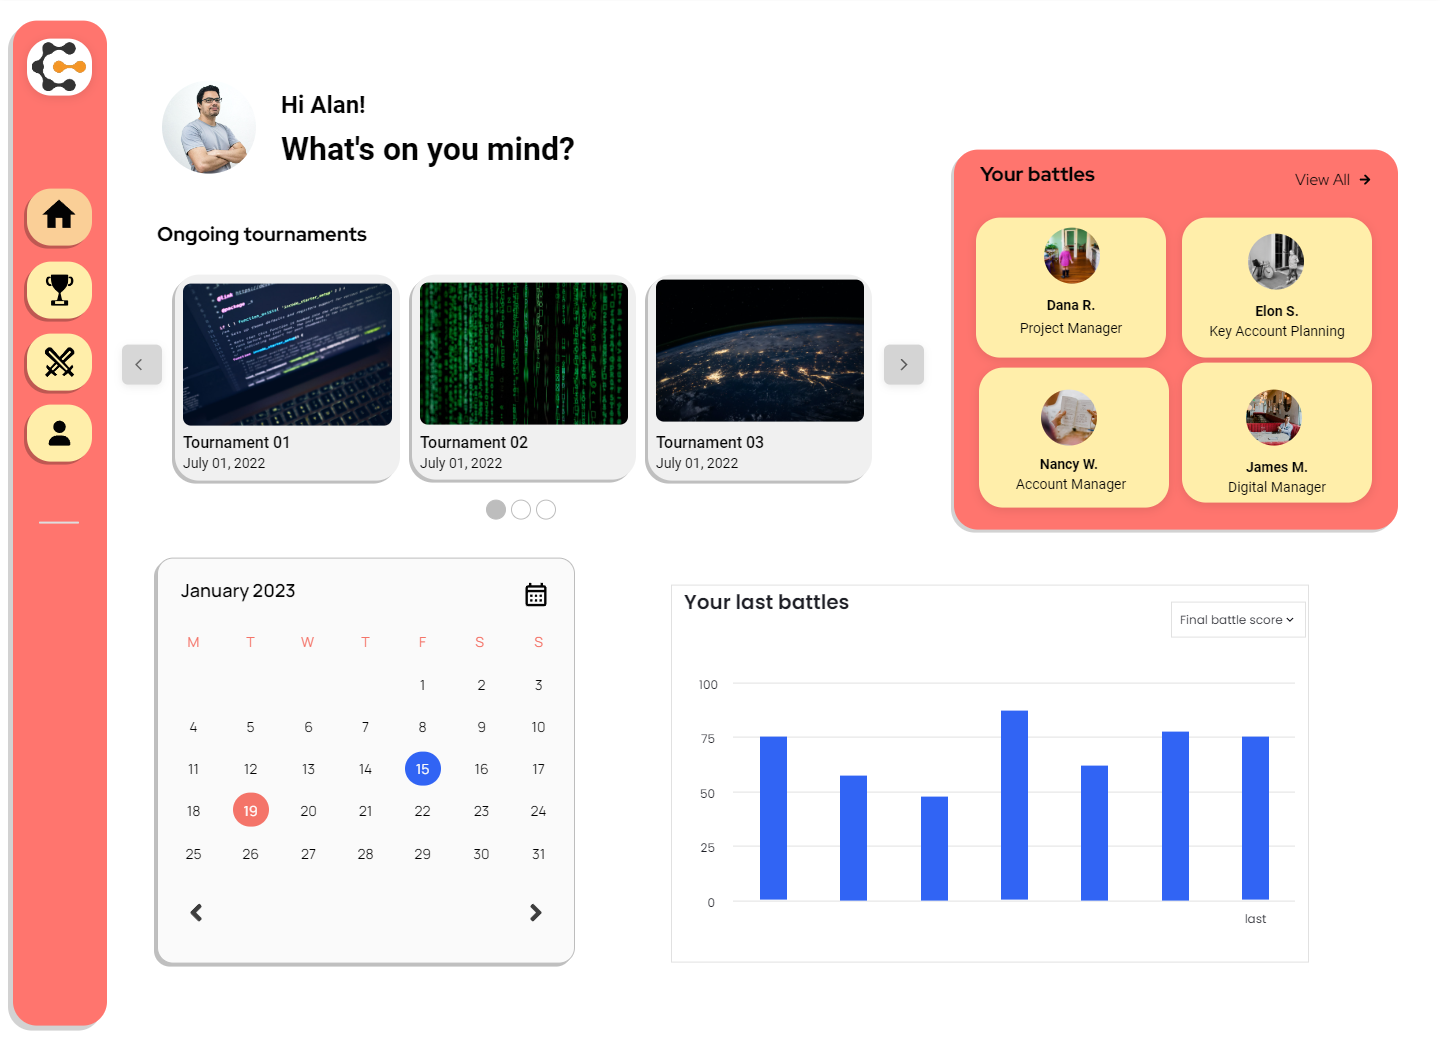
\includegraphics[width=1\textwidth]{Mockups/3_student_homepage.png}
    \caption{Home page from the perspective of an user logged as student}
    \label{fig:student_homepage}
\end{figure}
\newpage
\hfill \break
The picture above shows the home page of the CKB website. It contains different information depending on the role of the user who is visiting it: Figure \ref{fig:student_homepage} in particular presents the home page as it appears to a student. It displays the list of all tournaments and battles the student is participating in and a calendar showing upcoming deadlines.

The educator's version of the page shows instead the list of all tournaments and battles he is managing. \\ \\ \\ \\

\begin{figure}[H]
    \centering
    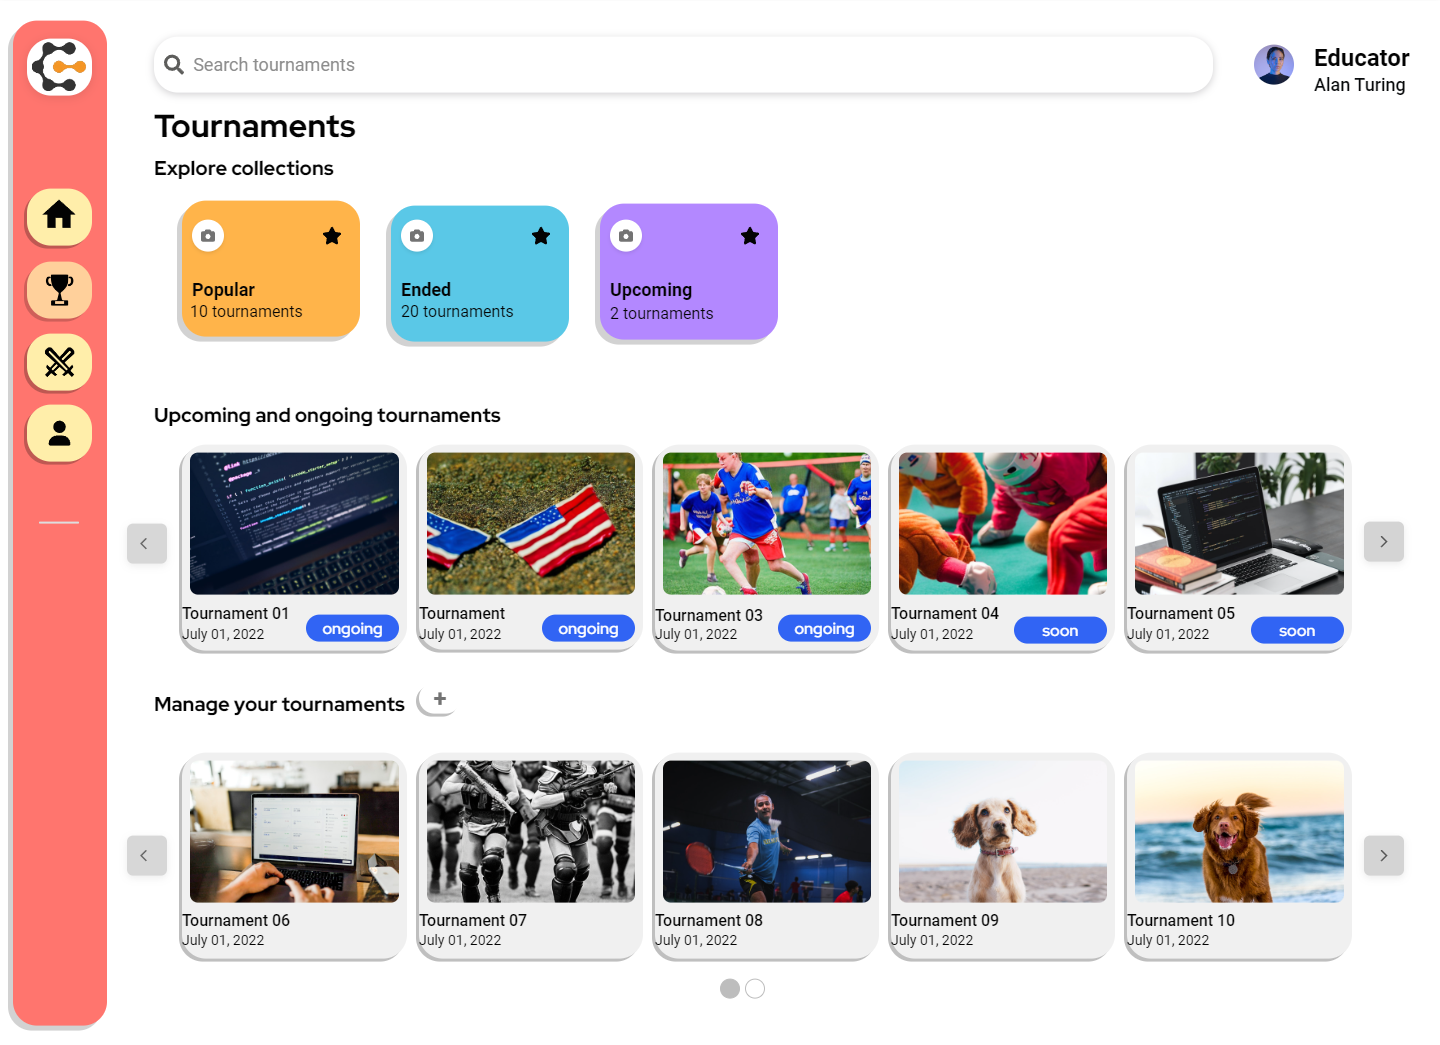
\includegraphics[width=1\textwidth]{Mockups/5_educator_tournaments.png}
    \caption{Tournaments page from the perspective of an user logged as educator}
\end{figure}
\newpage
\hfill \break
The tournaments section contains the list of all past, ongoing and upcoming tournaments. User can click on a specific tournament to navigate to the tournament's specific page. \\ \\ \\ \\ \\ \\

\begin{figure}[H]
    \centering
    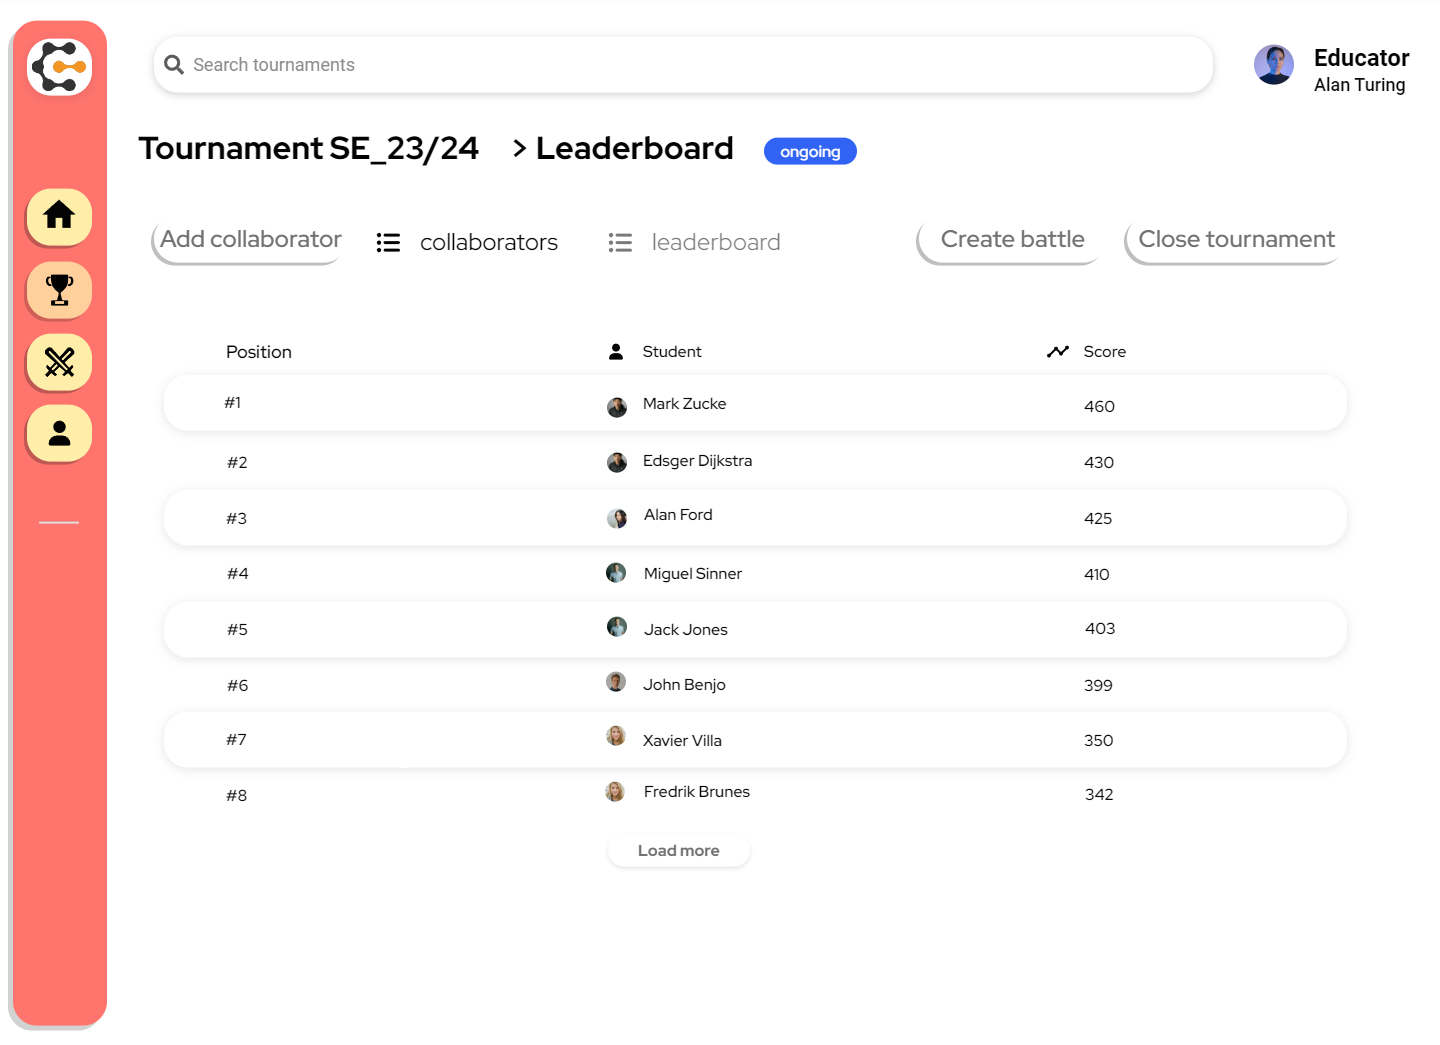
\includegraphics[width=1\textwidth]{Mockups/8_educator_tournament_leaderboard.png}
    \caption{"Leaderboard" tab available to both educators and students to check the ranking in tournament}
    \label{fig:leaderboard}
\end{figure}
\newpage
\hfill \break
The tournament page allows the users to visualize the personal rank of students participating in it. Figure \ref{fig:leaderboard} shows in particular how the leaderboard will be displayed to an educator.  \\ \\ \\ \\ \\ \\

\begin{figure}[H]
    \centering
    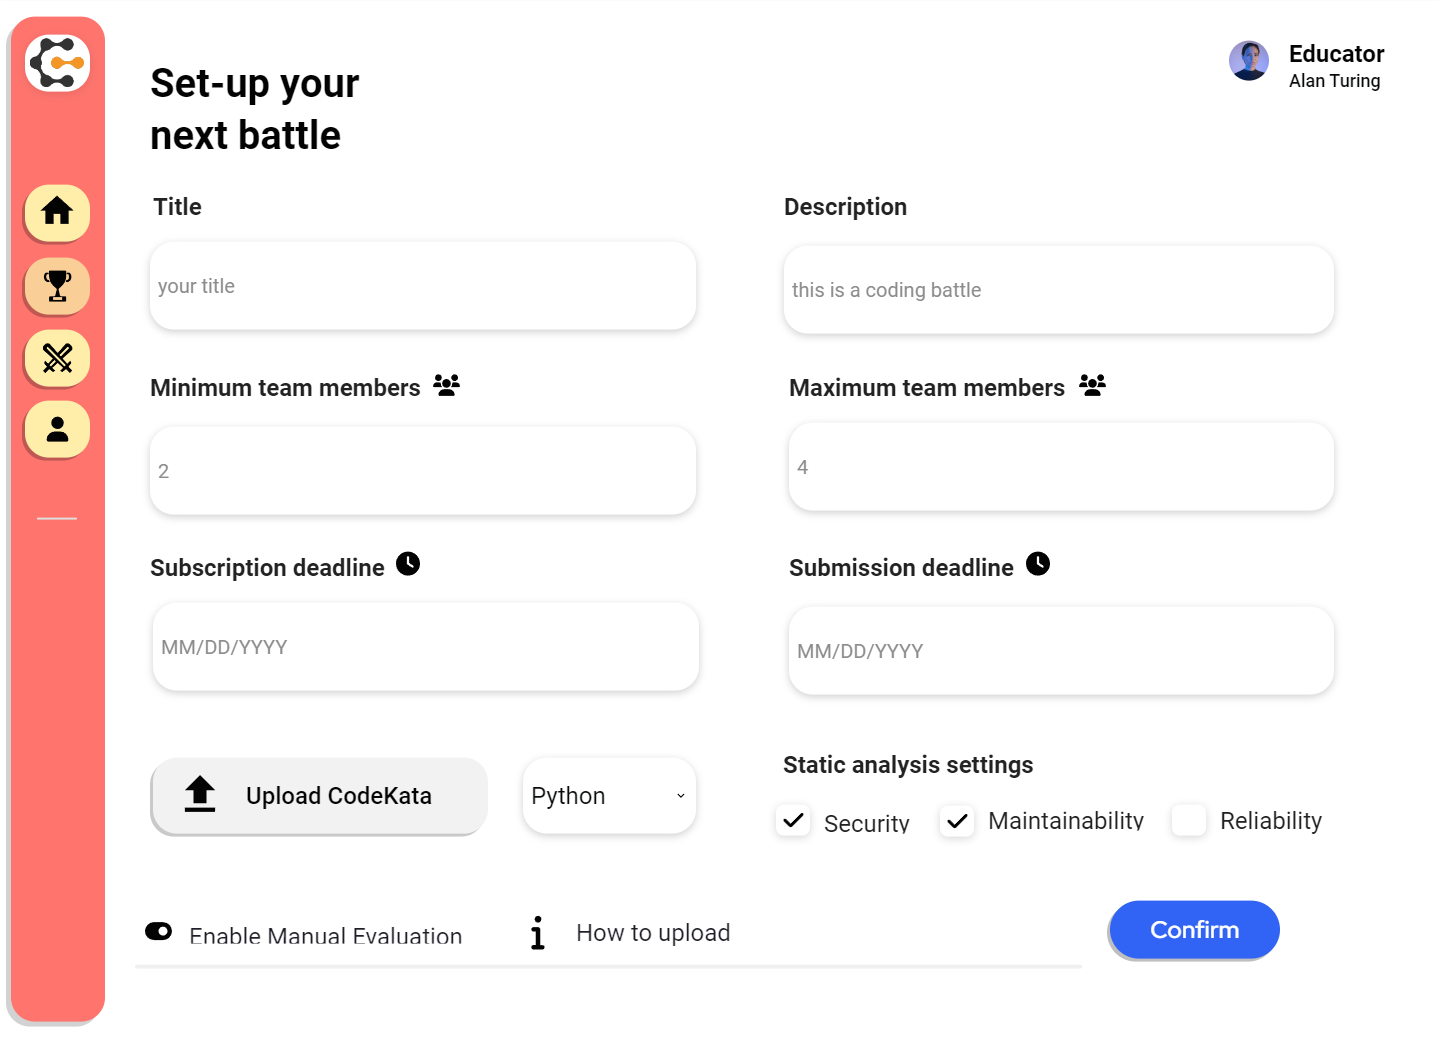
\includegraphics[width=1\textwidth]{Mockups/10_educator_create_battle.png}
    \caption{Page used from educators to create a new battle}
\end{figure}
\newpage
\hfill \break
The create battle functionality is available only to educators and allows them to insert all the relevant information about the challenge and to upload the Code Kata files. \\ \\ \\ \\ \\ \\

\begin{figure}[H]
    \centering
    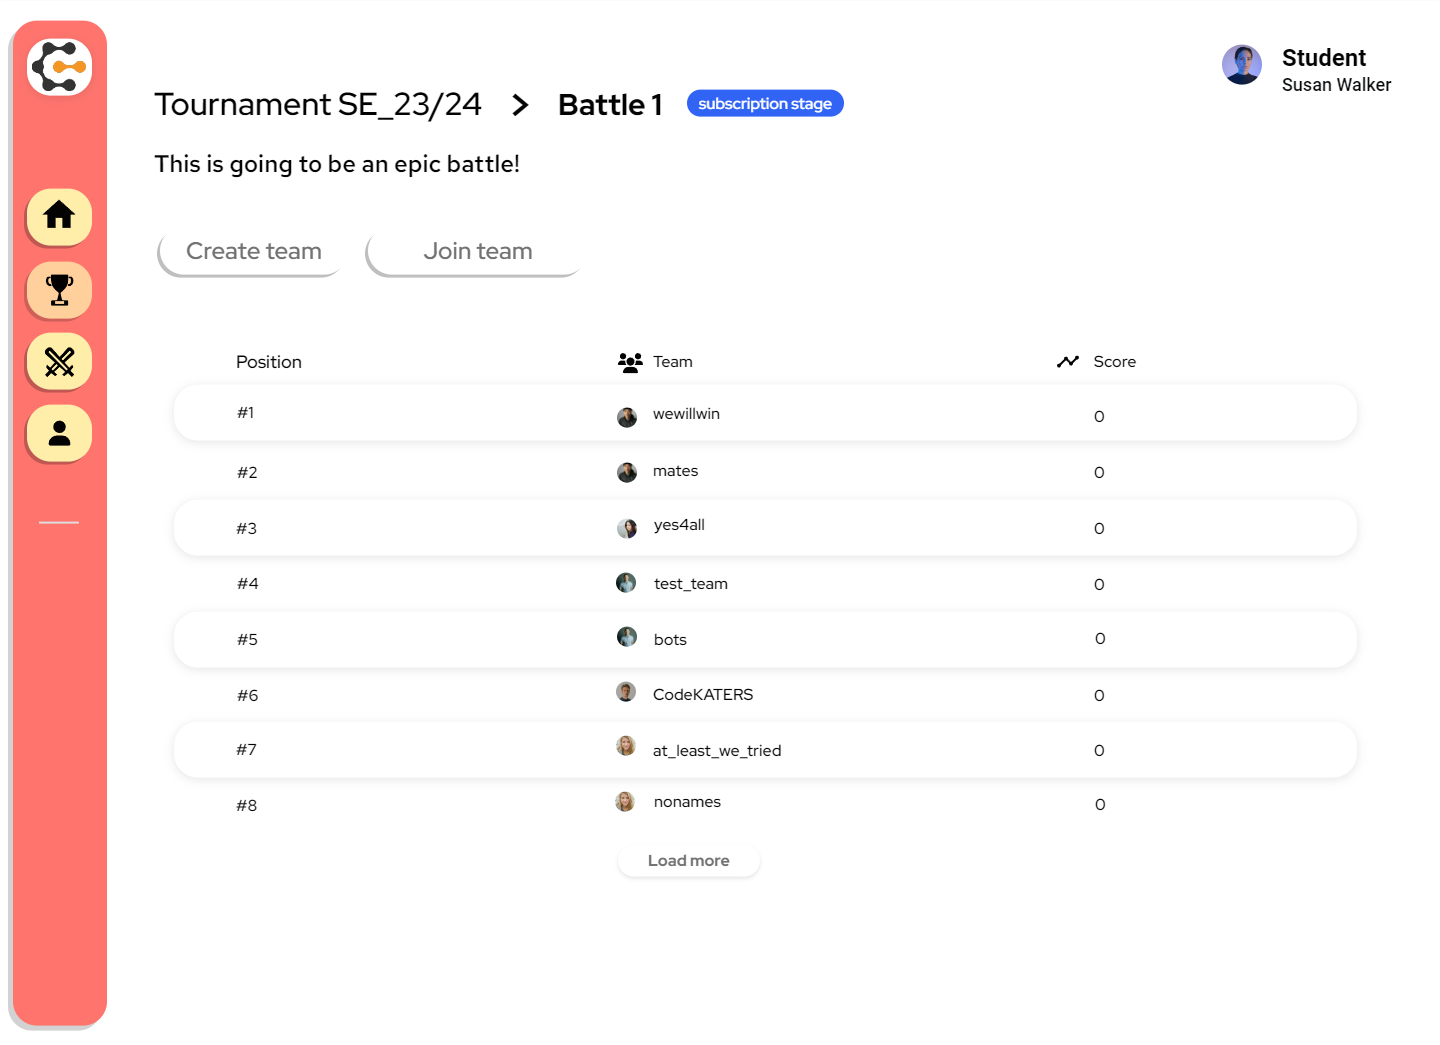
\includegraphics[width=1\textwidth]{Mockups/11_student_battle_subscription.png}
    \caption{Page used from students to subscribe to a battle}
\end{figure}
\newpage
\hfill \break
Another key service of the platform is provided by the battle page. It allows educators to access the battle management functionality. Students, through this page, can instead subscribe to the battle. This section is also used to visualize the battle's leaderboard to all the users. \\ \\ \\ \\ \\

\begin{figure}[H]
    \centering
    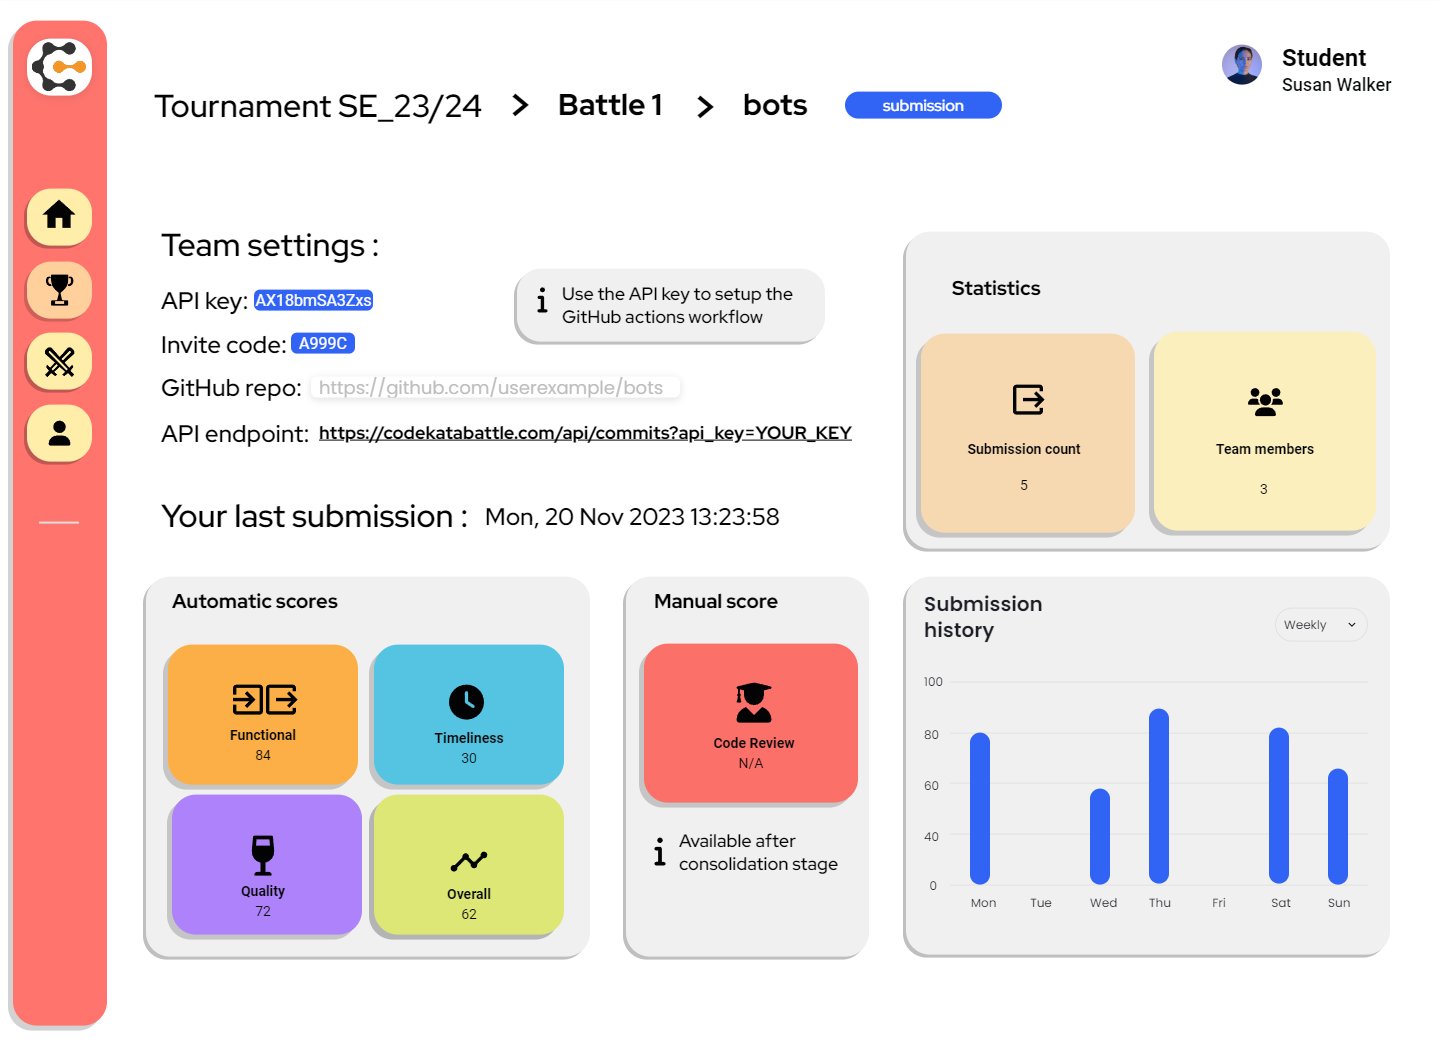
\includegraphics[width=1\textwidth]{Mockups/15_student_team.png}
    \caption{Page used from students to manage the settings of their team and to check submissions information}
\end{figure}
\newpage
\hfill \break
The team page is used by students to check and configure the settings of their team (e.g. GitHub repository related information). It also allows them to visualize details about their last submission.

Educators will also access the same page to review the code and assign a manual score to the team.

\subsubsection{Hardware Interfaces}
The software does not require any other hardware interface different than personal computers or smartphones equipped with modern browser from which users can access the platform.

\subsubsection{Software Interfaces}
Some of the functionalities provided by the system exploit specific interfaces to work. These are:
\begin{itemize}
    \item \textbf{GitHub interface}: the system must be able to interface with GitHub API to create the original repository for each battle and to pull code submissions.
    \item \textbf{Static analysis tools}: some of the aspects that have to be evaluated require the execution of static analysis methods over the provided code. System achieves this by interfacing with external tools that provide this functionality. These services must support the set of languages allowed by the CKB platform and the analysis of specific code quality aspects such as security, maintainability and reliability.
\end{itemize}

Moreover, in order to be notified about the submission of a new solution, the system itself must expose a \textbf{REST endpoint} that will be invoked by the automated GitHub Actions workflow set up by each team on their repository.

\newpage
\subsubsection{Communication Interfaces}
Given that the majority of the system's services are provided through the platform's website and REST API calls, no other protocol than HTTP should be needed. Anyway, it is worth mentioning that part of the communication between the system and user is achieved through notifications sent via mail using an external mail service provider.
\newpage

\subsection{Functional Requirements}
The main requirements the system has to fulfill are the following:
\begin{enumerate}[label=$\bullet$ \textbf{R\arabic*:}]
    \item System shall allow user to register as educator or student.
    \item System shall allow user to log in.
    \item System shall allow educator to create a tournament.
    \item System shall allow educator (tournament creator) to set the name of the tournament.
    \item System shall allow educator (tournament creator) to set the subscription deadline of the tournament.
    \item System shall notify all students enrolled to the platform about a newly created tournament.
    \item System shall allow educator (tournament creator) to end the tournament.
    \item System shall allow educator (tournament creator) to add another educator as collaborator to the tournament.
    \item System shall allow educator (tournament creator or collaborator) to create a battle for the tournament.
    \item System shall allow educator (battle creator) to upload the Code Kata of the battle.
    \item System shall allow educator (battle creator) to set minimum and maximum number of students per group allowed for the battle.
    \item System shall allow educator (battle creator) to set the registration deadline of the battle.
    \item System shall allow educator (battle creator) to set the submission deadline of the battle.
    \item System shall allow educator (battle creator) to enable/disable optional manual evaluation for the battle.
    \item System shall allow educator (battle creator) to select relevant aspects of code quality to be extracted through static analysis.
    \item System shall notify all users enrolled to a tournament about a newly created battle.
    \item The system shall be able to perform static analysis on submitted code utilizing third-party static code analysis tools and services.
    \item System shall create the GitHub repository of a battle as soon as the registration phase closes, sending its link to all involved students.
    \item System shall assign to each submission sent before the submission deadline a score (natural number between 0 and 100) combining correctness, timeliness and code quality \textit{as soon as possible}.
    \item System shall allow educator (battle creator) to set a manual score (natural number between 0 and 100) to the last valid team’s submission during the consolidation stage of the battle.
    \item System shall compute a final score combining automatic and manual score (if available) for each team if manual evaluation is enabled.
    \item System shall update the battle teams’ ranks right after a new score is available.
    \item System shall notify all students participating to the battle about the availability of the final battle rank.
    \item System shall update the tournament students’ scores as the sum of all the battle scores received during the tournament once the final battle rank becomes available.
    \item System shall notify all involved users about the availability of the tournament student’s final rank.
    \item System shall allow all users to see the list of ongoing tournaments.
    \item System shall allow all users to see all tournaments’ ranks.
    \item System shall allow all users to see all battles' ranks.
    \item System should manage every ranking (tournament or battle) in a way that it represents the correct order of students/teams within its context, from the ones with the highest score to the ones with the lowest.
    \item System shall allow student to enroll to a tournament within the subscription deadline.
    \item System shall allow student to create a team within the registration deadline.
    \item System shall allow student (team creator) to set the team name.
    \item System shall allow student (team creator) to set the privacy of the group.
    \item System shall allow student to join a team \textit{only} before the registration deadline.
    \item System shall allow \textit{only} students who know the correct invite code to join private groups.
    \item System shall allow team members to set their the repository URL.
    \item System shall generate a unique API token for each team.
    \item System should offer an external API which, when invoked, will notify the platform about a new commit on a team’s GitHub repository.
    \item System shall allow the educator to access the code of the submitted solutions.
    \item System shall generate a unique invite code for each team.
    \item System shall allow educator (battle creator) to close the consolidation stage of the battle if manual evaluation is enabled.
    \item System shall allow students to see the latest score of their team.
\end{enumerate}
\newpage

\subsubsection{Use cases}
\textbf{Shared perspective}
\begin{figure}[H]
    \hspace{-40px}
    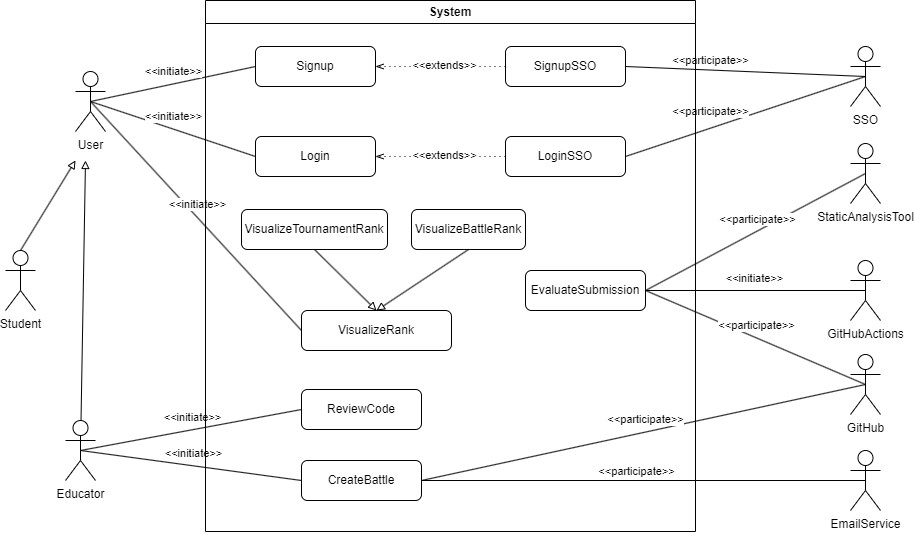
\includegraphics[scale=0.5]{Diagrams/use_case_both.png}
    \caption{Shared scenarios use case diagram}
\end{figure}
\begin{center}
    \hspace{-5px}
    \begin{tabular}{ |c|m{10cm}| }
        \hline
        \textbf{ID} & UC1 \\
        \hline
        \textbf{Name} & Signup \\
        \hline
        \textbf{Actors} & User, Email Service \\
        \hline
        \textbf{Entry conditions} &
        \begin{itemize}
            \item User is connected to the platform’s website
            \item User selected the option to register to the service
        \end{itemize} \\
        \hline
        \textbf{Event flow} &
        \begin{enumerate}
            \item User inserts the required information
            \item User flags the “Sign up as student” checkbox if he/she wants to sign up as a student, otherwise leaves it unchecked. In the case of a student, is also asked to provide its GitHub username
            \item User clicks on the “Sign up” button
            \item System checks user data
            \item System sends a confirmation email to the user
            \item User confirms the email address by clicking on the link inside the verfication email
        \end{enumerate} \\
        \hline
        \textbf{Exit conditions} &
        \begin{itemize}
            \item System adds the new user to its internal database
            \item User is logged in and redirected to the Home page
        \end{itemize} \\
        \hline
        \textbf{Exceptions} & 
        \begin{itemize}
            \item The email provided by the user is already in use for another account of the same type (student or educator)
            \item Some text field is left empty
            \item In the case of a student, does not exist any GitHub account corresponding to the provided username
        \end{itemize} 
        In all previous cases the registration is rejected and an error message is displayed on the page \\
        \hline
    \end{tabular}
    \begin{figure}[H]
        \hspace{52px}
        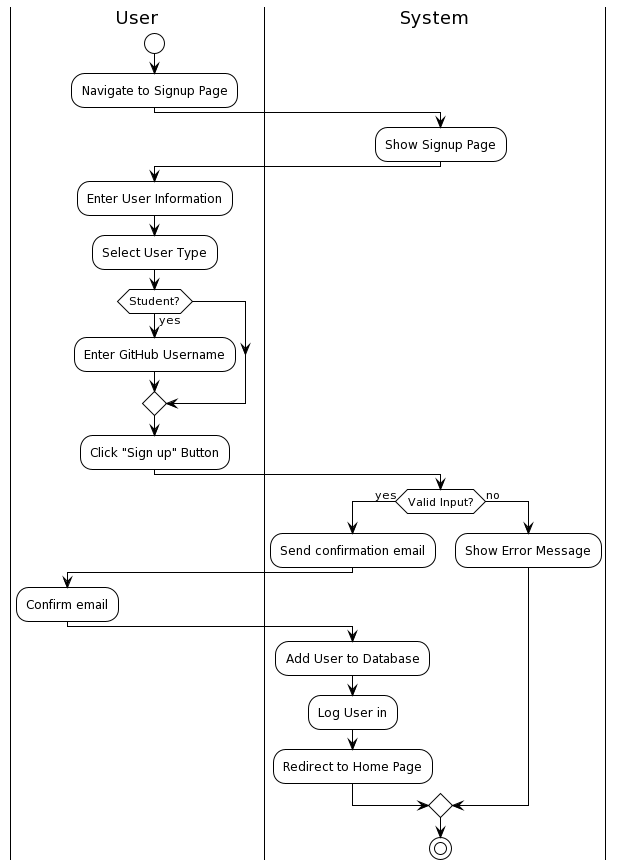
\includegraphics[scale=0.5]{Diagrams/activity_signup.png}
        \caption{Sign up use case activity diagram}
    \end{figure}
    \begin{tabular}{ |c|m{10cm}| }
        \hline
        \textbf{ID} & UC2 \\
        \hline
        \textbf{Name} & SignupSSO \\
        \hline
        \textbf{Actors} & User, Identity provider \\
        \hline
        \textbf{Entry conditions} &
        \begin{itemize}
            \item User is connected to the platform’s website
            \item User selected the option to register to the service
        \end{itemize} \\
        \hline
        \textbf{Event flow} &
        \begin{enumerate}
            \item User clicks on the icon of the identity provider he/she wants to sign up through
            \item SSO provides to the system the information it needs for the user’s registration
            \item Inside a new page, the user needs to click one of two buttons to specify whether he/she wants to sign up as a student or as an educator. In the case of a student, is also asked to provide its GitHub username
            \item System checks user data
        \end{enumerate} \\
        \hline
        \textbf{Exit conditions} &
        \begin{itemize}
            \item System adds the new user to its internal database
            \item User is logged in and redirected to the Home page
        \end{itemize} \\
        \hline
        \textbf{Exceptions} & 
        \begin{itemize}
            \item The email provided by the user is already in use for another account of the same type (student or educator)
            \item In the case of a student, does not exist any GitHub account corresponding to the provided username
        \end{itemize} 
        In all previous cases the registration is rejected and an error message is displayed on the page \\
        \hline
    \end{tabular}
    \begin{figure}[H]
        \hspace{25px}
        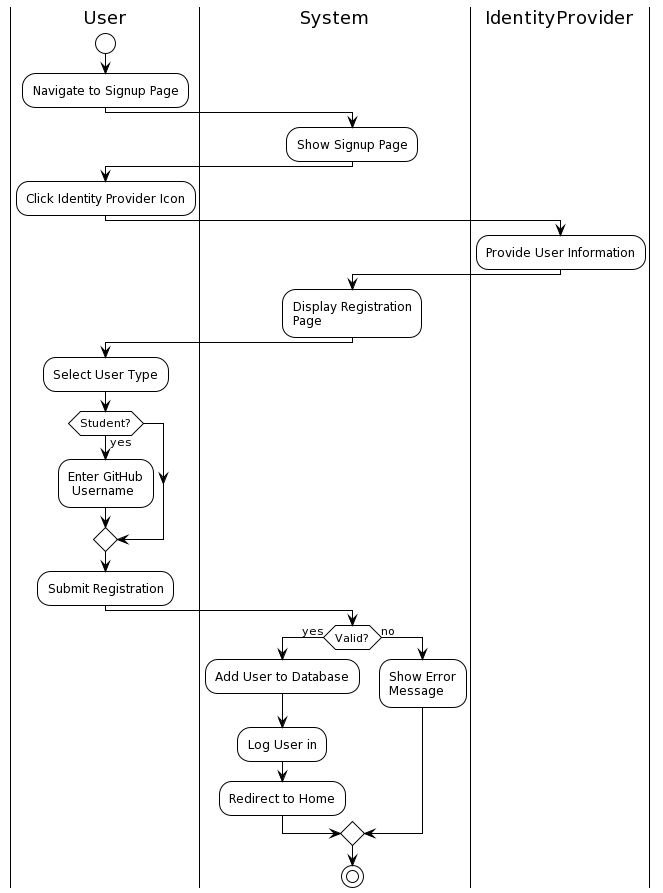
\includegraphics[scale=0.5]{Diagrams/activity_signupsso.png}
        \caption{Sign up through SSO use case activity diagram}
    \end{figure}
    \begin{tabular}{ |c|m{10cm}| }
        \hline
        \textbf{ID} & UC3 \\
        \hline
        \textbf{Name} & Login \\
        \hline
        \textbf{Actors} & User \\
        \hline
        \textbf{Entry conditions} &
        \begin{itemize}
            \item User is connected to the platform’s website
            \item User selected the option to log in
            \item User has already registered to the service
        \end{itemize} \\
        \hline
        \textbf{Event flow} &
        \begin{enumerate}
            \item User fills username and password fields
            \item User clicks on the “Log in” button
            \item System checks the validity of the provided credentials
        \end{enumerate} \\
        \hline
        \textbf{Exit conditions} &
        \begin{itemize}
            \item User is logged in and redirected to the Home page
        \end{itemize} \\
        \hline
        \textbf{Exceptions} & 
        \begin{itemize}
            \item The provided credentials do not correspond to any of the accounts registered on the platform
            \item Some text field is left empty
        \end{itemize} 
        In all previous cases the log in request is rejected and an error message is displayed on the page \\
        \hline
    \end{tabular}
    \begin{figure}[H]
        \hspace{57px}
        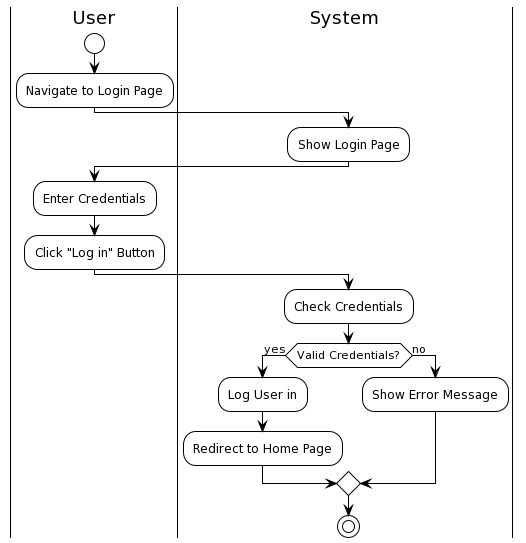
\includegraphics[scale=0.5]{Diagrams/activity_login.png}
        \caption{Log in use case activity diagram}
    \end{figure}
    \begin{tabular}{ |c|m{10cm}| }
        \hline
        \textbf{ID} & UC4 \\
        \hline
        \textbf{Name} & LoginSSO \\
        \hline
        \textbf{Actors} & User, Identity provider \\
        \hline
        \textbf{Entry conditions} &
        \begin{itemize}
            \item User is connected to the platform’s website
            \item User selected the option to log in
            \item User has already registered to the service
        \end{itemize} \\
        \hline
        \textbf{Event flow} &
        \begin{enumerate}
            \item User clicks on the icon of the Identity provider he/she signed up with
            \item SSO provides to the system the information it needs for the user’s authentication
            \item System checks user validity
        \end{enumerate} \\
        \hline
        \textbf{Exit conditions} &
        \begin{itemize}
            \item User is logged in and redirected to the Home page
        \end{itemize} \\
        \hline
        \textbf{Exceptions} & 
        \begin{itemize}
            \item User selects a different identity provider with respect to the one he/she initially used to register to the platform
        \end{itemize} 
        In the previous case the log in request is rejected and an error message is displayed on the page \\
        \hline
    \end{tabular}
    \begin{figure}[H]
        \hspace{15px}
        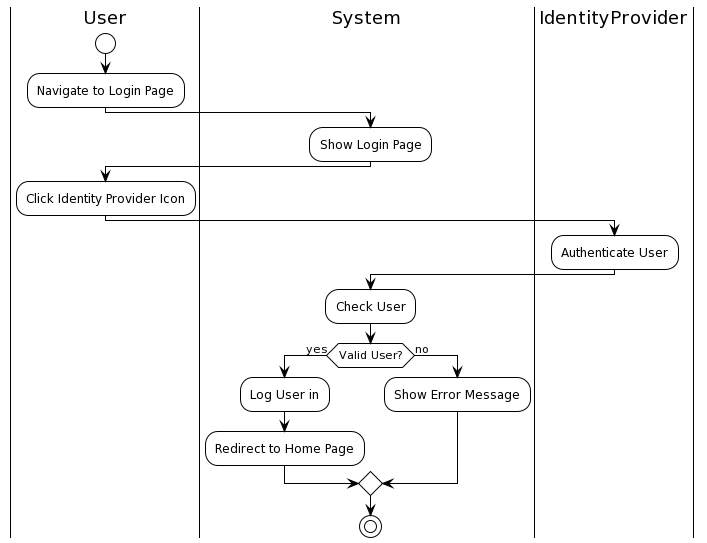
\includegraphics[scale=0.5]{Diagrams/activity_loginsso.png}
        \caption{Log in through SSO use case activity diagram}
    \end{figure}
    \begin{tabular}{ |c|m{10cm}| }
        \hline
        \textbf{ID} & UC5 \\
        \hline
        \textbf{Name} & CreateBattle \\
        \hline
        \textbf{Actors} & Educator, GitHub, Email Service \\
        \hline
        \textbf{Entry conditions} &
        \begin{itemize}
            \item Educator is logged in
            \item Educator has created or is a collaborator of the tournament in the context of which he/she wants to create the new battle in
            \item Educator has already prepared the Code Kata zip file
        \end{itemize} \\
        \hline
        \textbf{Event flow} &
        \begin{enumerate}
            \item Educator navigates to the tournaments page
            \item Educator selects the tournament from his/her “Manage your tournaments” list
            \item Educator clicks the “Create battle” button
            \item Educator inserts all the needed information and uploads the Code Kata
            \item Educator clicks the “Confirm” button
            \item Educator is redirected to the tournament’s page
            \item System checks the validity of the provided information and project files
            \item System notifies all the students enrolled into the tournament about the new battle via the Email Service
        \end{enumerate} \\
        \hline
    \end{tabular}
    \newpage
    \begin{tabular}{ |c|m{10cm}| }
        \hline
        \textbf{Exit conditions} &
        \begin{itemize}
            \item System adds the new battle to the tournament’s battles list and students can subscribe to it until the registration deadline
            \item System creates the repository for the challenge via GitHub API when the subscription deadline is met. System sends an email to all the students subscribed to the battle with the URL of the repository to fork
            \item Emails to students are correctly dispatched
        \end{itemize} \\
        \hline
        \textbf{Exceptions} & 
        \begin{itemize}
            \item The provided title has already been used for another battle of the same tournament 
            \item Some text field is left empty
            \item The uploaded Code Kata is not correctly structured
        \end{itemize} 
        In all previous cases the battle creation request is refused and an error message is shown in the page \\
        \hline
    \end{tabular}
    \begin{figure}[H]
        \hspace{7px}
        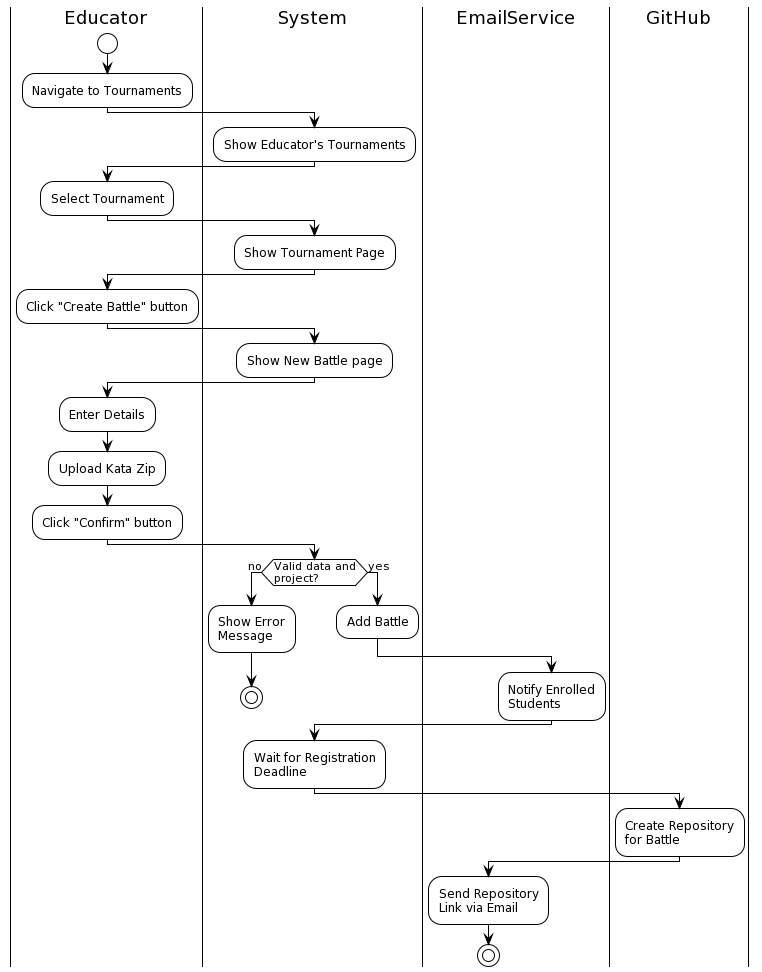
\includegraphics[scale=0.5]{Diagrams/activity_createbattle.png}
        \caption{Battle creation use case activity diagram}
    \end{figure}
    \begin{tabular}{ |c|m{10cm}| }
        \hline
        \textbf{ID} & UC6 \\
        \hline
        \textbf{Name} & VisualizeTournamentRank \\
        \hline
        \textbf{Actors} & User \\
        \hline
        \textbf{Entry conditions} &
        \begin{itemize}
            \item User is logged in
        \end{itemize} \\
        \hline
        \textbf{Event flow} &
        \begin{enumerate}
            \item User navigates to the tournaments page
            \item User inputs the name of the tournament of interest in the dedicated searchbox
            \item User selects the right tournament
            \item User clicks the “Leaderboard” button
        \end{enumerate} \\
        \hline
        \textbf{Exit conditions} &
        \begin{itemize}
            \item System shows the page containing the tournament’s ranking
        \end{itemize} \\
        \hline
        \textbf{Alternative} & 
            1a. User directly selects the tournament from the ones shown inside his/her tournaments page or home page \\
        \hline
        \textbf{Exceptions} & 
        \begin{itemize}
            \item Tournaments state is not “Ongoing” or “Ended”
        \end{itemize} 
        In the previous case the “Leaderboard” button will not be clickable \\
        \hline
    \end{tabular}
    \begin{figure}[H]
        \hspace{30px}
        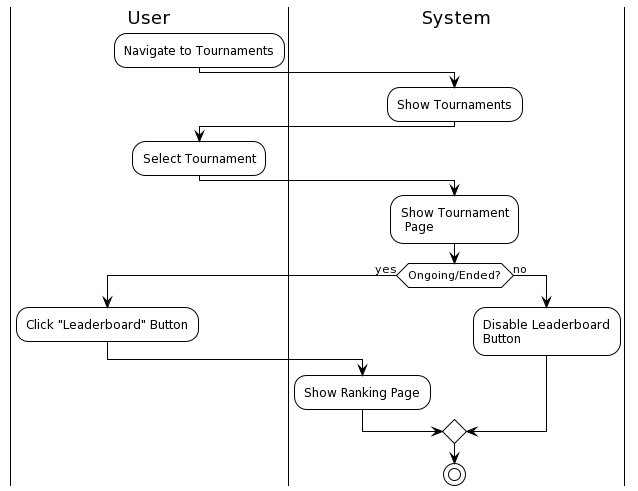
\includegraphics[scale=0.5]{Diagrams/activity_visualizetournamentrank.png}
        \caption{Tournament ranking's visualization use case activity diagram}
    \end{figure}
    \begin{tabular}{ |c|m{10cm}| }
        \hline
        \textbf{ID} & UC7 \\
        \hline
        \textbf{Name} & VisualizeBattleRank \\
        \hline
        \textbf{Actors} & User \\
        \hline
        \textbf{Entry conditions} &
        \begin{itemize}
            \item User is logged in
        \end{itemize} \\
        \hline
        \textbf{Event flow} &
        \begin{enumerate}
            \item User navigates to the tournaments page
            \item User inputs the name of the tournament of interest in the dedicated searchbox
            \item User selects the right tournament
            \item User selects the battle of interest from the tournament’s battle list
        \end{enumerate} \\
        \hline
        \textbf{Exit conditions} &
        \begin{itemize}
            \item System shows the page containing the battle’s ranking
        \end{itemize} \\
        \hline
        \textbf{Alternative} & 
            1a. User directly selects the battle from the ones shown in the context of his/her home page \\
        \hline
        \textbf{Exceptions} & 
        \begin{itemize}
            \item Battle is in Registration Phase
        \end{itemize} 
        In the previous case the battle's ranking will simply show the list of teams that subscribed till now \\
        \hline
    \end{tabular}
    \begin{figure}[H]
        \hspace{90px}
        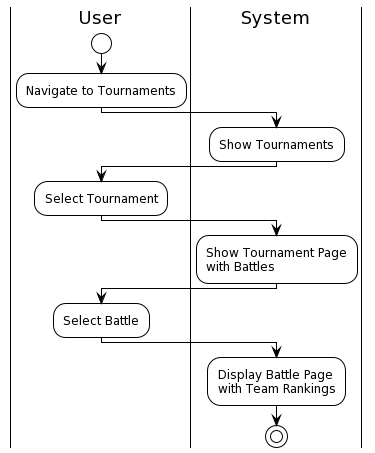
\includegraphics[scale=0.5]{Diagrams/activity_visualizebattlerank.png}
        \caption{Battle ranking's visualization use case activity diagram}
    \end{figure}
    \begin{tabular}{ |c|m{10cm}| }
        \hline
        \textbf{ID} & UC8 \\
        \hline
        \textbf{Name} & EvaluateSubmission \\
        \hline
        \textbf{Actors} & GitHub Actions, GitHub, Static Analysis tool \\
        \hline
        \textbf{Entry conditions} &
        \begin{itemize}
            \item Team has forked the battle's repository (once per team)
            \item GitHub Actions workflow is setup (once per team)
            \item Team’s repository is setup in the team’s settings page (once per team)
            \item A new commit is pushed into team’s GitHub repository
        \end{itemize} \\
        \hline
        \textbf{Event flow} &
        \begin{enumerate}
            \item GitHub Actions performs a request directed to the system’s API endpoint, including the relative API token of the team as an additional parameter of the request
            \item System checks the validity of the token and retrieves the corresponding repository URL
            \item System pulls the code of the new submission directly from GitHub via API
            \item System computes a score for timeliness by comparing the timestamp of the request with the one corresponding to the start of the submission phase of the battle
            \item System computes a score for correctness by executing all the test cases provided and comparing the results with the expected ones
            \item If specified from the battle creator, the system provides the code for the evaluation to the external static analysis tool which will assign a score for each of the code quality aspects selected at battle creation time
        \end{enumerate} \\
        \hline
    \end{tabular}
    \newpage
    \begin{tabular}{ |c|m{10cm}| }
        \hline
        \textbf{Exit conditions} &
        \begin{itemize}
            \item System computes an overall score by averaging the results of all the previous evaluations and updates the team’s score and rank
        \end{itemize} \\
        \hline
        \textbf{Exceptions} & 
        \begin{itemize}
            \item GitHub Actions workflow is not correctly setup, the system’s endpoint receives a request with a token that does not correspond to any of the teams subscribed to the battle
            \item Repository’s url is not correctly setup in the team’s settings page, system is not able to retrieve the code
        \end{itemize} 
        In all previous cases the new submission is simply ignored by the system \\
        \hline
    \end{tabular}
    \begin{figure}[H]
        \hspace{15px}
        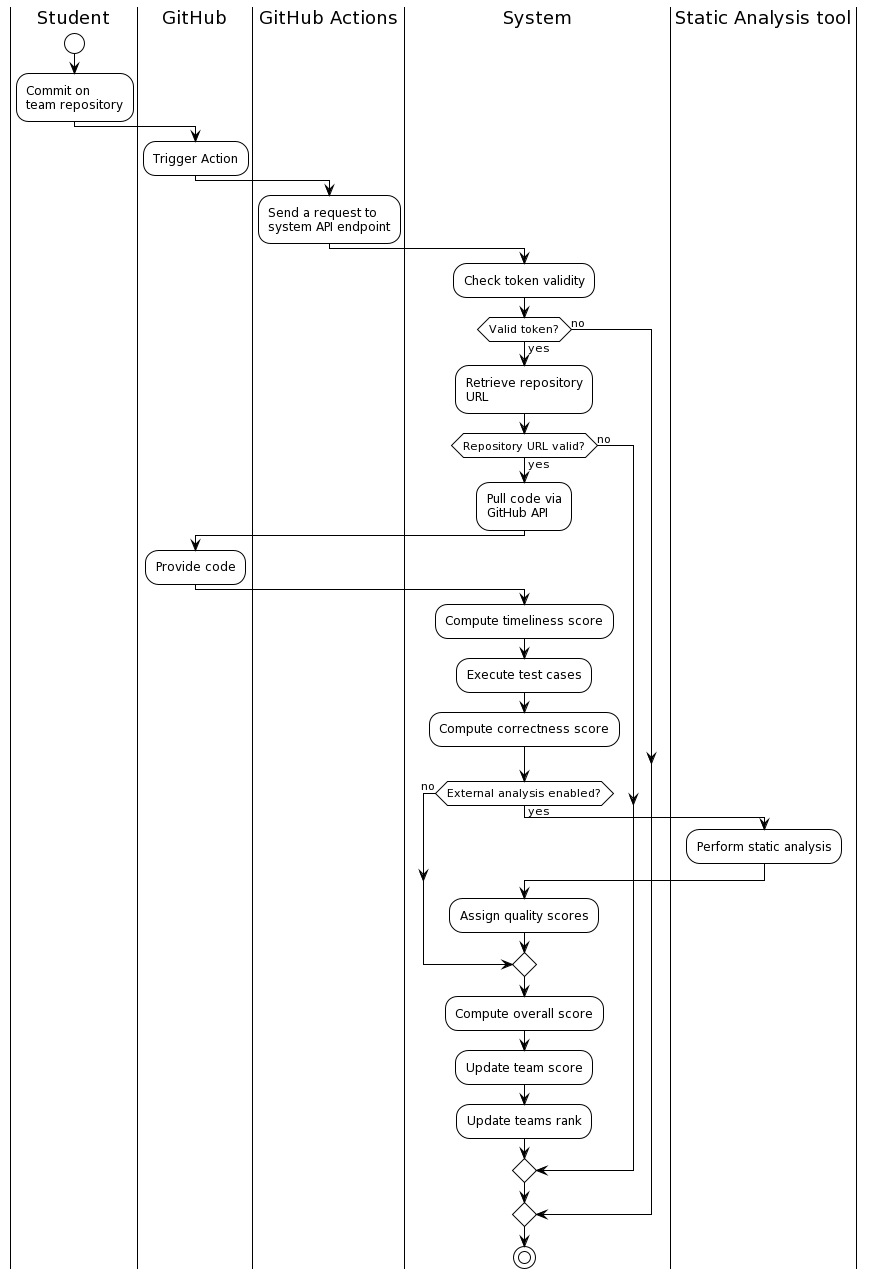
\includegraphics[scale=0.4]{Diagrams/activity_evaluatesubmission.png}
        \caption{Submission evaluation use case activity diagram}
    \end{figure}
    \begin{tabular}{ |c|m{10cm}| }
        \hline
        \textbf{ID} & UC9 \\
        \hline
        \textbf{Name} & ReviewCode \\
        \hline
        \textbf{Actors} & Educator, GitHub \\
        \hline
        \textbf{Entry conditions} &
        \begin{itemize}
            \item Educator is logged in
            \item Battle is in Consolidation Stage
        \end{itemize} \\
        \hline
        \textbf{Event flow} &
        \begin{enumerate}
            \item Educator navigates to the tournament section
            \item Educator selects the right tournament
            \item Educator selects the battle of interest
            \item Educator selects a team from the battle’s ranking
            \item Educator clicks the link to the team’s GitHub repository to inspect the code
            \item Educator provides a score by inputting it inside the dedicated textbox
            \item Educator clicks the “Confirm” button
        \end{enumerate} \\
        \hline
        \textbf{Exit conditions} &
        \begin{itemize}
            \item System saves the new manual score in its database and computes the final battle score as the average between the new score and the automatic evaluation results
        \end{itemize} \\
        \hline
        \textbf{Alternative} & 
            1a. Educator directly selects the battle from the ones shown in the context of his/her home page \\
        \hline
        \textbf{Exceptions} & 
        \begin{itemize}
            \item The score text field is left empty or contains something that is not an integer number between 0 and 100
        \end{itemize} 
        In this case the score registration request is rejected and an error message is shown \\
        \hline
    \end{tabular}
    \begin{figure}[H]
        \hspace{10px}
        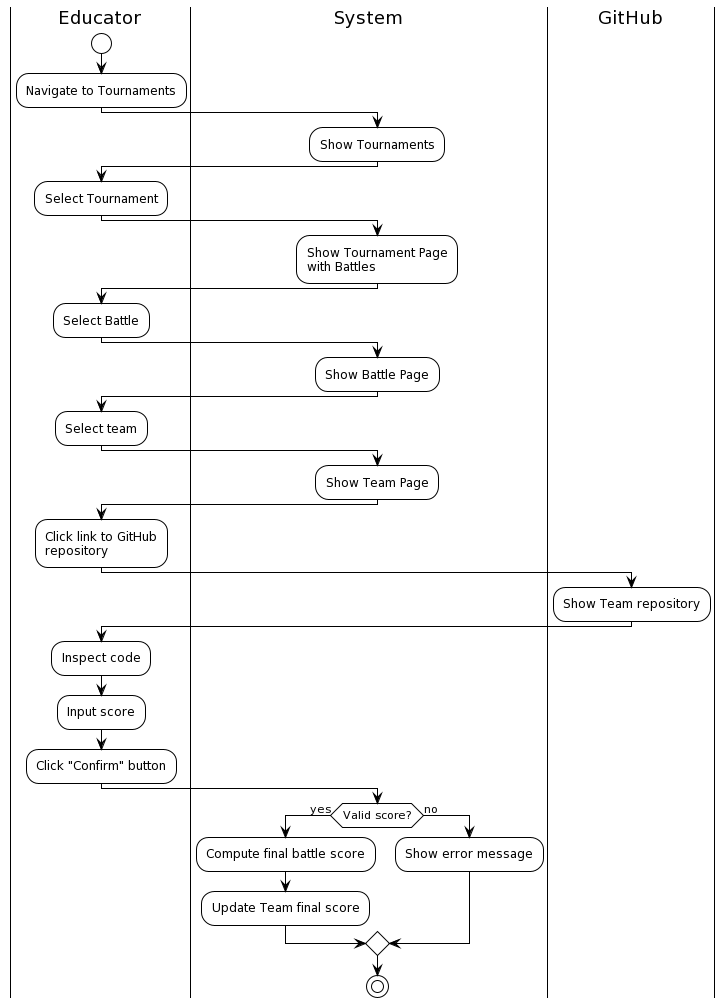
\includegraphics[scale=0.5]{Diagrams/activity_reviewcode.png}
        \caption{Code review use case activity diagram}
    \end{figure}
\end{center}

\textbf{Student perspective}
\begin{figure}[H]
    \hspace{40px}
    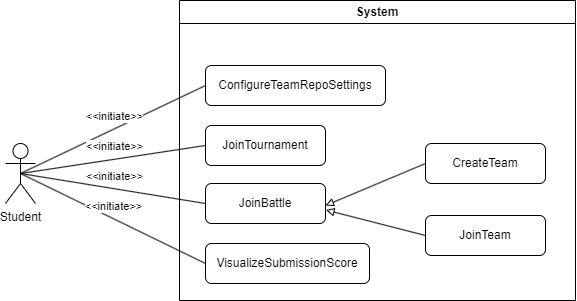
\includegraphics[scale=0.5]{Diagrams/use_case_student.png}
    \caption{Students' scenarios use case diagram}
\end{figure}
\begin{center}
    \begin{tabular}{ |c|m{10cm}| }
        \hline
        \textbf{ID} & UC10 \\
        \hline
        \textbf{Name} & JoinTournament \\
        \hline
        \textbf{Actors} & Student \\
        \hline
        \textbf{Entry conditions} &
        \begin{itemize}
            \item Student is logged in
        \end{itemize} \\
        \hline
        \textbf{Event flow} &
        \begin{enumerate}
            \item Student navigates to the tournaments section
            \item System shows the list of tournaments the student is enrolled in and the list of all available tournaments in the platform
            \item Student clicks on one of the tournaments in the list of available tournaments
            \item Student is redirected to the page of the tournament containing the list of all students currently enrolled
            \item Student clicks on “Enroll”
        \end{enumerate} \\
        \hline
        \textbf{Exit conditions} &
        \begin{itemize}
            \item Student is correctly enrolled into the tournament
        \end{itemize} \\
        \hline
    \end{tabular}
    \begin{figure}[H]
        \hspace{80px}
        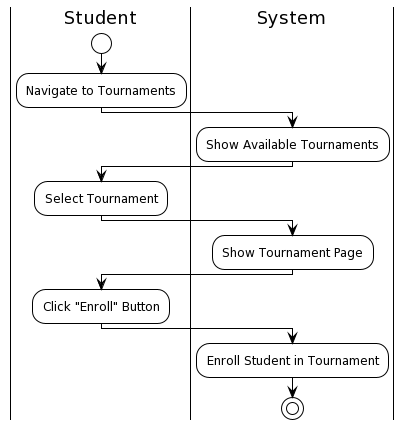
\includegraphics[scale=0.5]{Diagrams/activity_jointournament.png}
        \caption{Joining a tournament use case activity diagram}
    \end{figure}
    \begin{tabular}{ |c|m{10cm}| }
        \hline
        \textbf{ID} & UC11 \\
        \hline
        \textbf{Name} & CreateTeam \\
        \hline
        \textbf{Actors} & Student \\
        \hline
        \textbf{Entry conditions} &
        \begin{itemize}
            \item Student is logged in
            \item Studen has already enrolled to the tournament
        \end{itemize} \\
        \hline
        \textbf{Event flow} &
        \begin{enumerate}
            \item Student navigates to the tournaments section
            \item System shows the list of tournaments the student is enrolled in
            \item Student clicks on one of the tournaments in the list
            \item Student is redirected to the page of the tournament containing the list of all the battles
            \item Student clicks on the battle he wants to participate in
            \item System redirects the student to the page of the battle
            \item Student clicks on the “Create Team” button
            \item System shows a pop-up with the team settings
            \item Student inputs the name of the team, selects the desired privacy setting and clicks on “Confirm”
        \end{enumerate} \\
        \hline
    \end{tabular}
    \newpage
    \begin{tabular}{ |c|m{10cm}| }
        \hline
        \textbf{Exit conditions} &
        \begin{itemize}
            \item Student is correctly enrolled into the battle with its new team
            \item System generates a unique invite API token and invite code valid for the team
            \item The battle’s page now shows a “Your team” button to manage the team settings
        \end{itemize} \\
        \hline
        \textbf{Exceptions} & 
        \begin{itemize}
            \item Student inputs a team name already in use for that battle
        \end{itemize} 
        In the previous case, the student is not able to create a team and a pop-up with a specific error message is shown \\
        \hline
    \end{tabular}
    \begin{figure}[H]
        \hspace{52px}
        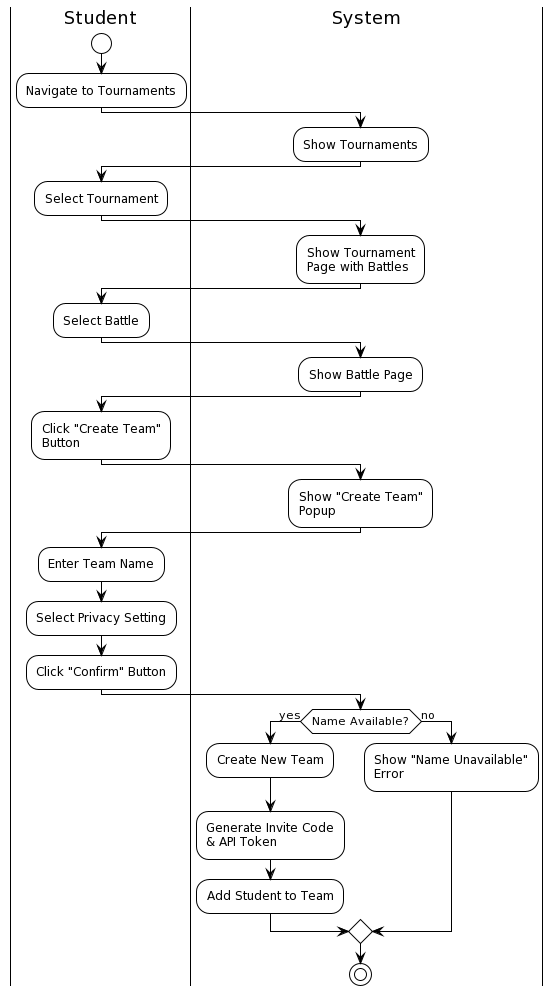
\includegraphics[scale=0.5]{Diagrams/activity_createteam.png}
        \caption{Team creation use case activity diagram}
    \end{figure}
    \begin{tabular}{ |c|m{10cm}| }
        \hline
        \textbf{ID} & UC12 \\
        \hline
        \textbf{Name} & JoinTeam \\
        \hline
        \textbf{Actors} & Student \\
        \hline
        \textbf{Entry conditions} &
        \begin{itemize}
            \item Student is logged in
            \item Studen has already enrolled to the tournament
        \end{itemize} \\
        \hline
        \textbf{Event flow} &
        \begin{enumerate}
            \item Student navigates to the tournaments section
            \item System shows the list of tournaments the student is enrolled in
            \item Student clicks on one of the tournaments in the list
            \item Student is redirected to the page of the tournament containing the list of all the battles
            \item Student clicks on the battle he wants to participate in
            \item System redirects the student to the page of the battle
            \item Student clicks on the “Join Team” button
            \item System shows a pop-up with 2 options and a input text field. The first options lets the user join a public team by name. The second option instead allows the user to join a team by invite code. The input field instead, asks for the team name or the invite code, depending on the checked option
            \item Student selects his preferred option, inputs the requested string and clicks on “Confirm”
        \end{enumerate} \\
        \hline
    \end{tabular}
    \newpage
    \begin{tabular}{ |c|m{10cm}| }
        \hline
        \textbf{Exit conditions} &
        \begin{itemize}
            \item Student is correctly enrolled into the battle with its new team
            \item The battle’s page now shows a “Your team” button to manage the team settings
        \end{itemize} \\
        \hline
        \textbf{Exceptions} & 
        \begin{itemize}
            \item Student tries to join a private team by name
            \item Student tries to join a team which has already reached maximum number of members
            \item Student inputs invalid team name or invite code
        \end{itemize} 
        In all the previous cases, the student is not able to join a team and a pop-up with a specific error message is shown \\
        \hline
    \end{tabular}
    \begin{figure}[H]
        \hspace{30px}
        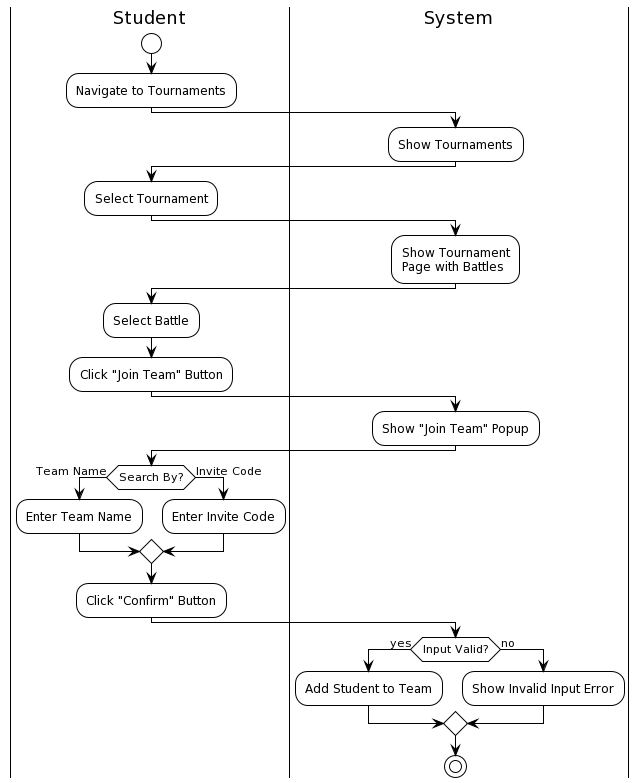
\includegraphics[scale=0.5]{Diagrams/activity_jointeam.png}
        \caption{Joining a team use case activity diagram}
    \end{figure}
    \begin{tabular}{ |c|m{10cm}| }
        \hline
        \textbf{ID} & UC13 \\
        \hline
        \textbf{Name} & ConfigureTeamRepoSettings \\
        \hline
        \textbf{Actors} & Student \\
        \hline
        \textbf{Entry conditions} &
        \begin{itemize}
            \item Student is logged in
            \item Student is already participating to a battle
        \end{itemize} \\
        \hline
        \textbf{Event flow} &
        \begin{enumerate}
            \item Student navigates to the tournaments section
            \item System shows the list of tournaments the student is enrolled in
            \item Student clicks on one of the tournaments in the list
            \item Student is redirected to the page of the tournament containing the list of all the battles
            \item Student clicks on the battle he wants to manage
            \item System redirects the student to the page of the battle
            \item Student clicks on “Your team” button
            \item System redirects the student to the page of the team
            \item Student can now visualize the team’s settings such as system’s API commit endpoint, team’s API token to setup the GitHub actions and the invite code. Student can also set the URL of the GitHub repository
        \end{enumerate} \\
        \hline
    \end{tabular}
    \newpage
    \begin{tabular}{ |c|m{10cm}| }
        \hline
        \textbf{Exit conditions} &
        \begin{itemize}
            \item Systems correctly saves the inputted GitHub repository URL
        \end{itemize} \\
        \hline
        \textbf{Exceptions} & 
        \begin{itemize}
            \item URL is invalid
        \end{itemize} 
        In the previous case, the system won’t accept the input and an error message is shown next to the input field \\
        \hline
    \end{tabular}
    \begin{figure}[H]
        \hspace{45px}
        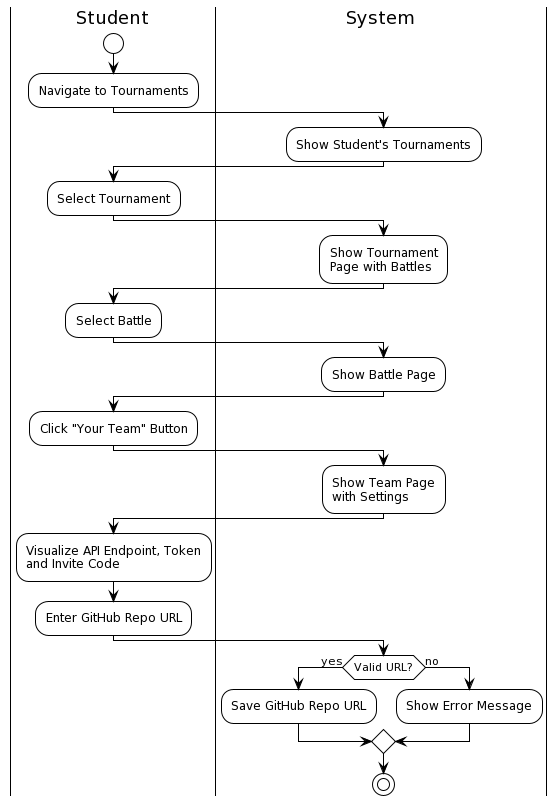
\includegraphics[scale=0.5]{Diagrams/activity_configureteamreposettings.png}
        \caption{Team settings' configuration use case activity diagram}
    \end{figure}
    \begin{tabular}{ |c|m{10cm}| }
        \hline
        \textbf{ID} & UC14 \\
        \hline
        \textbf{Name} & VisualizeSubmissionScore \\
        \hline
        \textbf{Actors} & Student \\
        \hline
        \textbf{Entry conditions} &
        \begin{itemize}
            \item Student is logged in
            \item Student is already participating to a battle
        \end{itemize} \\
        \hline
        \textbf{Event flow} &
        \begin{enumerate}
            \item Student navigates to the tournaments section
            \item System shows the list of tournaments the student is enrolled in
            \item Student clicks on one of the tournaments in the list
            \item Student is redirected to the page of the tournament containing the list of all the battles
            \item Student clicks on the battle he wants to check 
            \item System redirects the student to the page of the battle
            \item Student clicks on “Your Team” button
            \item System redirects the student to the page of the team
        \end{enumerate} \\
        \hline
        \textbf{Exit conditions} &
        \begin{itemize}
            \item System shows all the scores related to the last submission and some statistics about past scores
        \end{itemize} \\
        \hline
        \textbf{Exceptions} & 
        \begin{itemize}
            \item Team hasn’t submitted any solution yet
        \end{itemize} 
        In the previous case, the team page will show no scores about last submission \\
        \hline
    \end{tabular}
    \begin{figure}[H]
        \hspace{37px}
        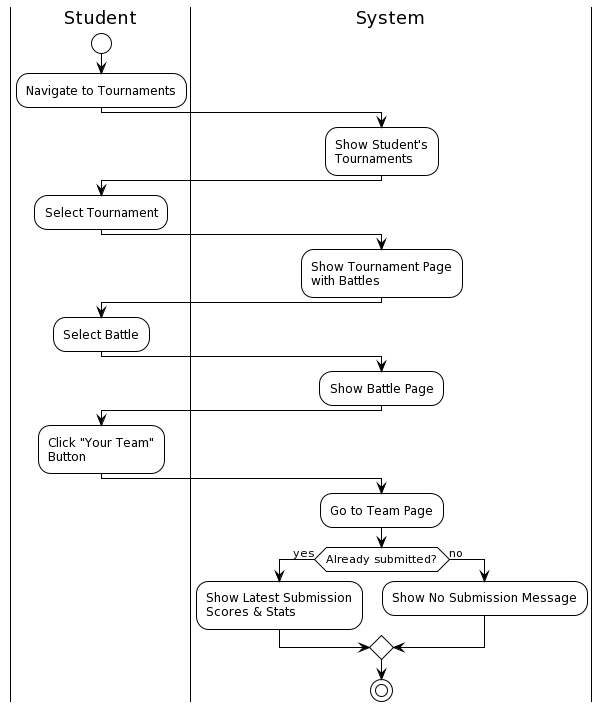
\includegraphics[scale=0.5]{Diagrams/activity_visualizesubmissionscore.png}
        \caption{Submission's score visualization use case activity diagram}
    \end{figure}
\end{center}
\newpage

\textbf{Educator perspective}
\begin{figure}[H]
    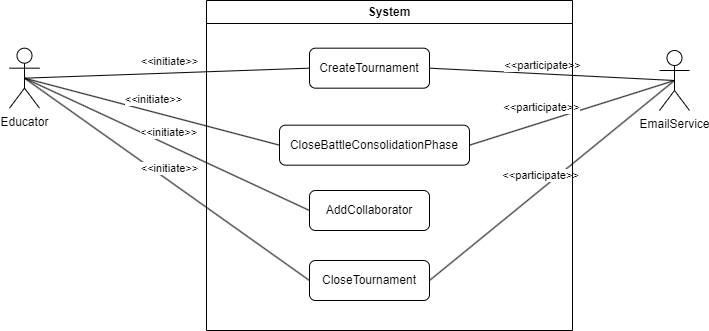
\includegraphics[scale=0.5]{Diagrams/use_case_educator.png}
    \caption{Educators' scenarios use case diagram}
\end{figure}
\begin{center}
    \begin{tabular}{ |c|m{10cm}| }
        \hline
        \textbf{ID} & UC15 \\
        \hline
        \textbf{Name} & CreateTournament \\
        \hline
        \textbf{Actors} & Educator, Email Service \\
        \hline
        \textbf{Entry conditions} &
        \begin{itemize}
            \item Educator is logged in
        \end{itemize} \\
        \hline
        \textbf{Event flow} &
        \begin{enumerate}
            \item Educator navigates to the tournaments section
            \item System shows the list of ongoing tournaments the educator is managing
            \item Educator clicks on the button next to the list to create a new tournament
            \item System prompts a pop-up asking the name and the subscription deadline
            \item Educator fills in with requested information and clicks on “Save”
            \item System notifies all the students of the platform about the new tournament via the Email Service
        \end{enumerate} \\
        \hline
        \textbf{Exit conditions} &
        \begin{itemize}
            \item System correctly creates the new tournament
            \item Educator is redirected to the new tournament page
            \item Emails to all the students are dispatched
        \end{itemize} \\
        \hline
        \textbf{Exceptions} & 
        \begin{itemize}
            \item Provided name is already in use
            \item Subscription deadline is invalid
        \end{itemize} 
        In all the previous cases, the educator is not able to create the tournament and a pop-up with a specific error message is shown \\
        \hline
    \end{tabular}
    \begin{figure}[H]
        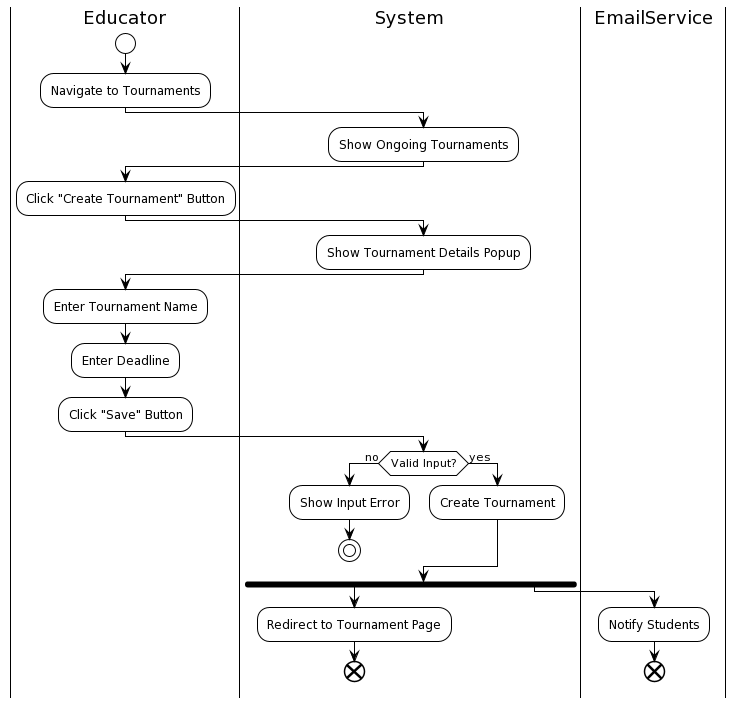
\includegraphics[scale=0.9]{Diagrams/activity_createtournament.png}
        \caption{Tournament creation use case activity diagram}
    \end{figure}
    \begin{tabular}{ |c|m{10cm}| }
        \hline
        \textbf{ID} & UC16 \\
        \hline
        \textbf{Name} & CloseTournament \\
        \hline
        \textbf{Actors} & Educator, Email Service \\
        \hline
        \textbf{Entry conditions} &
        \begin{itemize}
            \item Educator is logged in
            \item Educator is the creator of an ongoing tournament
        \end{itemize} \\
        \hline
        \textbf{Event flow} &
        \begin{enumerate}
            \item Educator navigates to the tournaments section
            \item System shows the list of ongoing tournaments the educator is managing
            \item Educator clicks on the tournament he is interested in
            \item System redirects the educator to the tournament’s page
            \item Educator clicks on the “Close Tournament” button 
            \item Systems notifies all the enrolled students about the end of the tournament
        \end{enumerate} \\
        \hline
        \textbf{Exit conditions} &
        \begin{itemize}
            \item Tournament ends correctly
            \item Emails to all the students are dispatched
        \end{itemize} \\
        \hline
        \textbf{Exceptions} & 
        \begin{itemize}
            \item Educator is trying to close a tournament with an ongoing battle
        \end{itemize} 
        In the previous case, the educator is not able to close the tournament and a pop-up with a specific error message is shown \\
        \hline
    \end{tabular}
    \begin{figure}[H]
        \hspace{7px}
        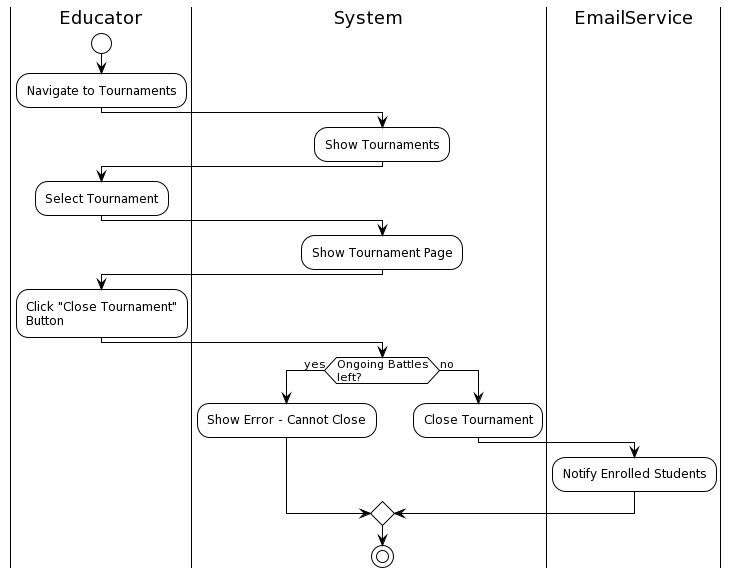
\includegraphics[scale=0.5]{Diagrams/activity_closetournament.png}
        \caption{Tournament closure use case activity diagram}
    \end{figure}
    \begin{tabular}{ |c|m{10cm}| }
        \hline
        \textbf{ID} & UC17 \\
        \hline
        \textbf{Name} & AddCollaborator \\
        \hline
        \textbf{Actors} & Educator \\
        \hline
        \textbf{Entry conditions} &
        \begin{itemize}
            \item Educator is logged in
            \item Educator is the creator of a tournament
        \end{itemize} \\
        \hline
        \textbf{Event flow} &
        \begin{enumerate}
            \item Educator navigates to the tournaments section
            \item System shows the list of ongoing tournaments the educator is managing
            \item Educator clicks on the tournament he is interested in
            \item System redirects the educator to the tournament’s page
            \item Educator clicks on the “Add Collaborator” button
            \item System prompts a pop-up asking the email of the collaborator to add
            \item Educator fills in the requested information and clicks on  “Save”
        \end{enumerate} \\
        \hline
        \textbf{Exit conditions} &
        \begin{itemize}
            \item New educator is correctly added to the tournament and can now create battles
        \end{itemize} \\
        \hline
        \textbf{Exceptions} & 
        \begin{itemize}
            \item Email does not belong to any educator registered to the platform
        \end{itemize} 
        In the previous case, the educator is not able to add the collaborator and a pop-up with a specific error message is shown \\
        \hline
    \end{tabular}
    \begin{figure}[H]
        \hspace{50px}
        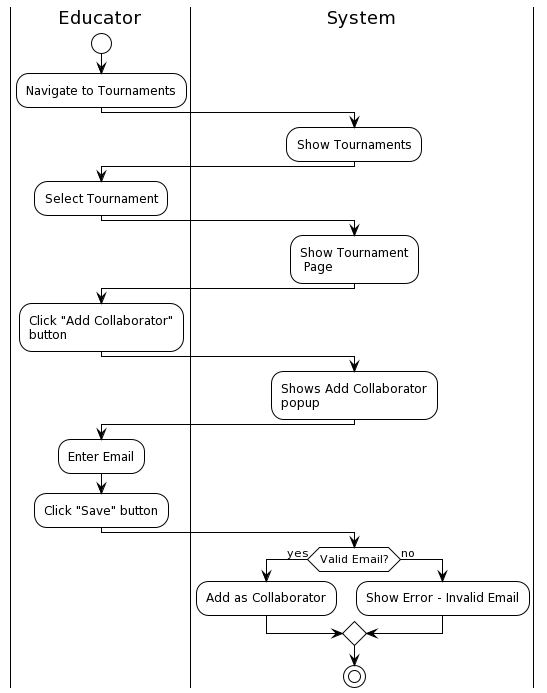
\includegraphics[scale=0.5]{Diagrams/activity_addcollaborator.png}
        \caption{Adding a collaborator to a tournament use case activity diagram}
    \end{figure}
    \begin{tabular}{ |c|m{10cm}| }
        \hline
        \textbf{ID} & UC18 \\
        \hline
        \textbf{Name} & CloseBattleConsolidationPhase \\
        \hline
        \textbf{Actors} & Educator, Email Service \\
        \hline
        \textbf{Entry conditions} &
        \begin{itemize}
            \item Educator is logged in
            \item Educator is the creator of a battle with the manual optional evaluation activated
            \item Battle's submission phase has expired
        \end{itemize} \\
        \hline
        \textbf{Event flow} &
        \begin{enumerate}
            \item Educator navigates to the tournaments section
            \item System shows the list of ongoing tournaments the educator is managing
            \item Educator clicks on the tournament he is interested in
            \item System redirects the educator to the tournament page, which contains the list of all the battles of the tournament
            \item Educator clicks on the battle he is the creator of
            \item System redirects the educator to the battle page
            \item Educator clicks on the “Close Consolidation” button
            \item System updates the personal tournament scores as the sum of all battle scores of the student obtained in the tournament
            \item System updates both the tournament rank and the final battle rank
            \item Systems notifies all the enrolled students into the battle about the availability of the battle scores
        \end{enumerate} \\
        \hline
    \end{tabular}
    \newpage
    \begin{tabular}{ |c|m{10cm}| }
        \hline
        \textbf{Exit conditions} &
        \begin{itemize}
            \item Battle is correctly closed, the new scores and ranks are updated
            \item Emails to all the students are dispatched
        \end{itemize} \\
        \hline
        \textbf{Exceptions} & 
        \begin{itemize}
            \item Educator is trying to close the consolidation stage of a battle without having completed the manual code evaluation
        \end{itemize} 
        In the previous case, the educator is not able to close the battle and a pop-up with a specific error message is shown, asking the educator to complete the evaluation first \\
        \hline
    \end{tabular}
    \begin{figure}[H]
        \hspace{-10px}
        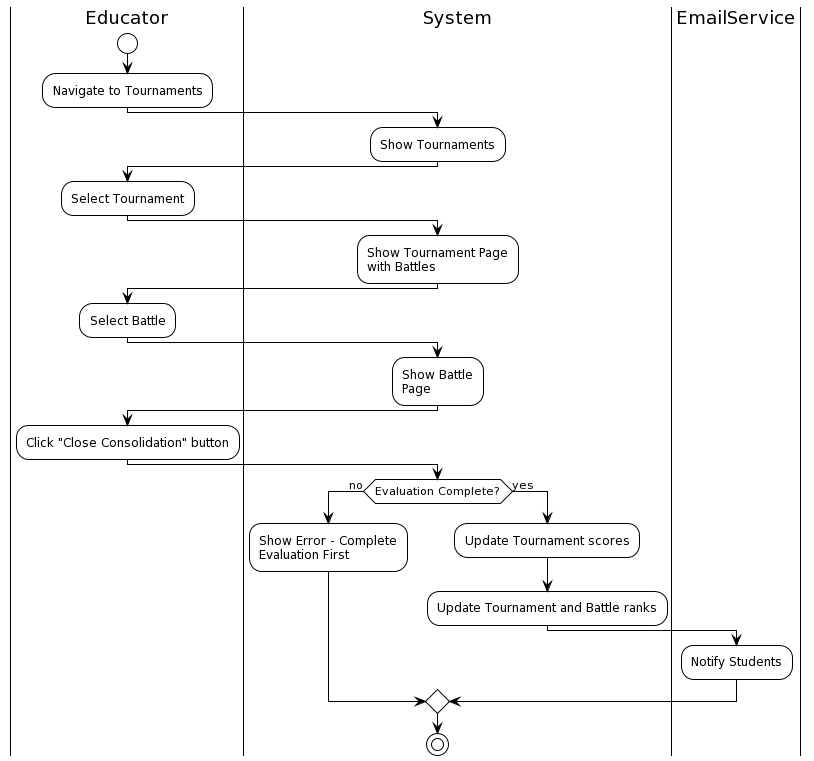
\includegraphics[scale=0.5]{Diagrams/activity_closebattleconsolidationphase.png}
        \caption{Close the consolidation phase of a battle use case activity diagram}
    \end{figure}
\end{center}

\subsubsection{Mapping on Use Cases}
\begin{center}
    \begin{tabular}{ |c|m{9cm}| }
        \hline
        \textbf{Use Case} & \textbf{Requirements} \\
        \hline
        UC1 & R1, R2 \\
        UC2 & R1, R2 \\
        UC3 & R2 \\
        UC4 & R2 \\
        UC5 & R9, R10, R11, R12, R13, R14, R15, R16, R18 \\
        UC6 & R26, R27 \\
        UC7 & R26, R28 \\
        UC8 & R17, R19, R22, R29, R37, R38, R39 \\
        UC9 & R20, R21, R39 \\
        UC10 & R26, R30 \\
        UC11 & R31, R32, R33, R37, R40 \\
        UC12 & R31, R34, R35 \\
        UC13 & R36, R37, R38, R40 \\
        UC14 & R42 \\
        UC15 & R3, R4, R5, R6 \\
        UC16 & R7, R25 \\
        UC17 & R8 \\
        UC18 & R21, R23, R24, R41 \\
        \hline
    \end{tabular}
\end{center}

\subsubsection{Mapping on Goals}
$\bullet$ \textbf{G1}: Allow students to participate to collaborative programming challenges
\begin{center}
    \begin{tabular}{ |m{3cm}|m{10cm}| }
        \hline
        \textbf{Requirements} 
        & \textbf{R1}: System shall allow user to register as educator or student \\
        & \textbf{R2}: System shall allow user to log in \\
        & \textbf{R6}: System shall notify all students enrolled to the platform about a newly created tournament \\
        & \textbf{R16}: System shall notify all users enrolled to a tournament about a newly created battle \\
        & \textbf{R18}: System shall create the GitHub repository of a battle as soon as the registration phase closes, sending its link to all involved students \\
        & \textbf{R26}: System shall allow all users to see the list of ongoing tournaments \\
        & \textbf{R30}: System shall allow student to enroll to a tournament within the subscription deadline \\
        & \textbf{R31}: System shall allow student to create a team within the registration deadline \\
        & \textbf{R32}: System shall allow student (team creator) to set the team name \\
        & \textbf{R33}: System shall allow student (team creator) to set the privacy of the group \\
        & \textbf{R34}: System shall allow student to join a team \textit{only} before the registration deadline \\
        & \textbf{R35}: System shall allow \textit{only} students who know the correct invite code to join private groups \\
        & \textbf{R36}: System shall allow team members to set their the repository URL \\
        & \textbf{R37}: System shall generate a unique API token for each team \\
        & \textbf{R38}: System should offer an external API which, when invoked, will notify the platform about a new commit on a team’s GitHub repository \\
        & \textbf{R40}: System shall generate a unique invite code for each team \\
        \hline
    \end{tabular}
    \begin{tabular}{ |m{3cm}|m{10cm}| }
        \hline
        \textbf{Domain \newline Assumptions} 
        & \textbf{D1}: Users have access to a stable and reliable internet connection to interact with the CKB platform \\
        & \textbf{D5}: Students are expected to engage in Code Kata Battles with integrity, without resorting to plagiarism or cheating (e.g. inviting more or different collaborators with respect to the ones inside the team) \\
        & \textbf{D6}: Maximum number of students per group an educator can set will always be bounded (e.g. less than 4) \\
        & \textbf{D7}: Every student has a GitHub account \\
        & \textbf{D8}: Students will fork the Code Kata GitHub repository once ready \\
        & \textbf{D9}: Students know how to setup a GitHub Actions worfkflow \\
        & \textbf{D10}: Only one student per group will perform the steps needed to set-up the team's repository and the GitHub Actions workflow \\
        & \textbf{D12}: Students use external communication channels \\
        \hline
    \end{tabular}
\end{center}
\newpage
$\bullet$ \textbf{G2}: Allow educators to create programming challenges
\begin{center}
    \begin{tabular}{ |m{3cm}|m{10cm}| }
        \hline
        \textbf{Requirements} 
        & \textbf{R1}: System shall allow user to register as educator or student \\
        & \textbf{R2}: System shall allow user to log in \\
        & \textbf{R3}: System shall allow educator to create a tournament \\
        & \textbf{R4}: System shall allow educator (tournament creator) to set the name of the tournament \\
        & \textbf{R5}: System shall allow educator (tournament creator) to set the subscription deadline of the tournament \\
        & \textbf{R7}: System shall allow educator (tournament creator) to end the tournament \\
        & \textbf{R8}: System shall allow educator (tournament creator) to add another educator as collaborator to the tournament \\
        & \textbf{R9}: System shall allow educator (tournament creator or collaborator) to create a battle for the tournament \\
        & \textbf{R10}: System shall allow educator (battle creator) to upload the Code Kata of the battle \\
        & \textbf{R11}: System shall allow educator (battle creator) to set minimum and maximum number of students per group allowed for the battle \\
        & \textbf{R12}: System shall allow educator (battle creator) to set the registration deadline of the battle \\
        & \textbf{R13}: System shall allow educator (battle creator) to set the submission deadline of the battle \\
        & \textbf{R14}: System shall allow educator (battle creator) to enable/disable optional manual evaluation for the battle \\
        & \textbf{R15}: System shall allow educator (battle creator) to select relevant aspects of code quality to be extracted through static analysis \\
        \hline
    \end{tabular}
    \begin{tabular}{ |m{3cm}|m{10cm}| }
        \hline
        \textbf{Domain \newline Assumptions} 
        & \textbf{D1}: Users have access to a stable and reliable internet connection to interact with the CKB platform \\
        & \textbf{D2}: Supported programming languages are limited to popular options like Java, Python and C++ \\
        & \textbf{D3}: Registered educators are all legitimate and verified \\
        & \textbf{D4}: Educators upload correct test cases and well-structured Code Kata projects \\
        & \textbf{D6}: Maximum number of students per group an educator can set will always be bounded (e.g. less than 4) \\
        \hline
    \end{tabular}
\end{center}        
$\bullet$ \textbf{G3}: Allow the system to automatically evaluate students' submissions
\begin{center}
    \begin{tabular}{ |m{3cm}|m{10cm}| }
        \hline
        \textbf{Requirements} 
        & \textbf{R17}: The system shall be able to perform static analysis on submitted code utilizing third-party static code analysis tools and services \\
        & \textbf{R18}: System shall create the GitHub repository of a battle as soon as the registration phase closes, sending its link to all involved students \\
        & \textbf{R19}: System shall assign to each submission sent before the submission deadline a score (natural number between 0 and 100) combining correctness, timeliness and code quality \textit{as soon as possible} \\
        & \textbf{R21}: System shall compute a final score combining automatic and manual score (if available) for each team if manual evaluation is enabled \\
        & \textbf{R36}: System shall allow team members to set their the repository URL \\
        & \textbf{R37}: System shall generate a unique API token for each team \\
        & \textbf{R38}: System should offer an external API which, when invoked, will notify the platform about a new commit on a team’s GitHub repository \\
        \hline
    \end{tabular}
    \begin{tabular}{ |m{3cm}|m{10cm}| }
        \hline
        \textbf{Domain \newline Assumptions} 
        & \textbf{D2}: Supported programming languages are limited to popular options like Java, Python and C++ \\
        & \textbf{D4}: Educators upload correct test cases and well-structured Code Kata projects \\
        & \textbf{D8}: Students will fork the Code Kata GitHub repository once ready \\
        & \textbf{D9}: Students know how to setup a GitHub Actions worfkflow \\
        & \textbf{D10}: Only one student per group will perform the steps needed to set-up the team's repository and the GitHub Actions workflow \\
        & \textbf{D11}: Static analysis tools are able to quantify the specified code quality aspects \\
        \hline
    \end{tabular}
\end{center} 
$\bullet$ \textbf{G4}: Allow educators to manually evaluate students' submissions
\begin{center}
    \begin{tabular}{ |m{3cm}|m{10cm}| }
        \hline
        \textbf{Requirements} 
        & \textbf{R1}: System shall allow user to register as educator or student \\
        & \textbf{R2}: System shall allow user to log in \\
        & \textbf{R13}: System shall allow educator (battle creator) to set the submission deadline of the battle \\
        & \textbf{R14}: System shall allow educator (battle creator) to enable/disable optional manual evaluation for the battle \\
        & \textbf{R20}: System shall allow educator (battle creator) to set a manual score (natural number between 0 and 100) to the last valid team’s submission during the consolidation stage of the battle \\
        & \textbf{R39}: System shall allow the educator to access the code of the submitted solutions \\
        & \textbf{R41}: System shall allow educator (battle creator) to close the consolidation stage of the battle if manual evaluation is enabled \\
        \hline
        \textbf{Domain \newline Assumptions} 
        & \textbf{D1}: Users have access to a stable and reliable internet connection to interact with the CKB platform \\
        & \textbf{D8}: Students will fork the Code Kata GitHub repository once ready \\
        & \textbf{D10}: Only one student per group will perform the steps needed to set-up the team's repository and the GitHub Actions workflow \\
        \hline
    \end{tabular}
\end{center} 
\newpage
$\bullet$ \textbf{G5}: Allow students to track their performance
\begin{center}
    \begin{tabular}{ |m{3cm}|m{10cm}| }
        \hline
        \textbf{Requirements} 
        & \textbf{R1}: System shall allow user to register as educator or student \\
        & \textbf{R2}: System shall allow user to log in \\
        & \textbf{R17}: The system shall be able to perform static analysis on submitted code utilizing third-party static code analysis tools and services \\
        & \textbf{R19}: System shall assign to each submission sent before the submission deadline a score (natural number between 0 and 100) combining correctness, timeliness and code quality \textit{as soon as possible} \\
        & \textbf{R20}: System shall allow educator (battle creator) to set a manual score (natural number between 0 and 100) to the last valid team’s submission during the consolidation stage of the battle \\
        & \textbf{R21}: System shall compute a final score combining automatic and manual score (if available) for each team if manual evaluation is enabled \\
        & \textbf{R22}: System shall update the battle teams’ ranks right after a new score is available \\
        & \textbf{R23}: System shall notify all students participating to the battle about the availability of the final battle rank \\
        & \textbf{R24}: System shall update the tournament students’ scores as the sum of all the battle scores received during the tournament once the final battle rank becomes available \\
        & \textbf{R25}: System shall notify all involved users about the availability of the tournament student’s final rank \\
        & \textbf{R27}: System shall allow all users to see all tournaments’ ranks \\
        & \textbf{R28}: System shall allow all users to see all battles' ranks \\
        & \textbf{R29}: System should manage every ranking (tournament or battle) in a way that it represents the correct order of students/teams within its context, from the ones with the highest score to the ones with the lowest \\
        & \textbf{R42}: System shall allow students to see the latest score of their team \\    
        \hline
    \end{tabular}
    \begin{tabular}{ |m{3cm}|m{10cm}| }
        \hline
        \textbf{Domain \newline Assumptions} 
        & \textbf{D1}: Users have access to a stable and reliable internet connection to interact with the CKB platform \\
        \hline
    \end{tabular}
\end{center} 

\subsection{Performance Requirements}
Even though the platform is not mission critical, should guarantee a smooth and appealing experience to all kind of users. Given the complexity of the overall project, several performance requirements for different aspects of the system can be identified:
\begin{itemize}
    \item \textit{Basic user interaction with the webapp}: response time for user actions like creating/joining a team, loading scoreboards, creating a tournament etc should be under 2 seconds for 90\% of requests under normal load.
    \item \textit{Space requirements}: a reasonable estimate of a project’s maximum size is about 40-50 MB. So, the system, to control the space usage, should limit the allowed projects sizes to 80 MB.
    \item \textit{Upload/download speed requirements}: given the previous estimate of project’s size, the system should guarantee a good throughput in terms of upload and download speed of the projects’ files. System should be able to reserve on average at least 8 Mb/s to each connection; this means that a project directory of 50 MB would take about 50 seconds to be downloaded. However, bandwidth of educator’s uploads should be prioritized. A pessimistic estimate with 1000 concurrent upload/download connections suggests that the systems needs at least a 10 Gb/s internet connection. Aggregating different Internet Service Providers may be considered to achieve greater bandwidths.
    \item \textit{Computational resources}: system should be sized to handle up to 100 simultaneous code submissions from different teams, providing a score within 20 seconds. Multiple CPUs with worker pooling approach will help in handling this kind of concurrency, dealing also with scalability issues.
    \item \textit{Notifications}: email notification should be able to reach all the recipients within 2 minutes.
\end{itemize}
These performance requirements will be taken in consideration also in choosing the external static analysis provider.

Moreover, given the different and independent performance requirements of all the functions involved, it is preferred to support each one with different machines or subsystems. In this way, the overall platform could still work with degraded performance affecting only a part of the functionalities.

The performance of the system could be improved following some basic strategies:
\begin{itemize}
    \item \textbf{Limit inbound API rate}: this will help in reducing commits from the same team (preventing also spam attacks).
    \item \textbf{Bound execution time}: terminate the evaluation of a submission after a timeout. This will help to prevent excessive resource consumption on tasks that should be quick to perform. 
\end{itemize}
In conclusion, it is important to mention again that even though the system is not providing an essential service to the user, it should offer a non stressful educational experience. Indeed, given the strict deadlines system, even a little delay in the submission can compromise the competition (which could potentially reflect into school marks of students), thus the overall purpose of the project.

\subsection{Design Constraints}
\subsubsection{Standards compliance}
There are several standards the system must comply with:
\begin{itemize}
    \item The web interface will comply with the latest versions of HTML, CSS and JavaScript standards.
    \item API will follow REST architectural constraints and use JSON data formats.
    \item Coordinated Universal Time (UTC) will be used to store timestamps in order to correctly show deadlines to user located in different time-zones.
\end{itemize}
\subsubsection{Hardware limitations}
The CDK platform has no strict hardware requirements, but should perform well on average smartphone or computer equipped with a modern web browser and a reliable internet connection.
\subsubsection{Privacy constraints}
Since the platform will need to ask the user for personal information like name, surname and email address, it needs to guarantee that this data will be processed and stored accordingly to the GDPR. Moreover, from the moment that the platform will also use cookies (e.g. to keep users authenticated), the system will need to get consent from visitors before placing cookies on their devices, in compliance with the EU ePrivacy regulations.
\subsubsection{Quality constraints}
User acceptance testing will measure task success rate and user satisfaction.

\subsection{Software System Attributes}
\subsubsection{Reliability}
Given the complexity of the project, reaching high reliability levels represents a challenge and a key to success for the product. Indeed, even though the systems performs many interactions with external actors and service providers, consistency and integrity of the overall platform should be guaranteed even in case of errors or unexpected conditions.
\subsubsection{Availability}
Service should be continuously available (24/7) to users, with little downtime and rapid service recovery. The overall service level target is 99.5\%, which corresponds nearly to 50 minutes of downtime per week. Planned maintenances should be communicated to users in advance, given the strict time requirements of the service offered by the platform.
\subsubsection{Usability}
The platform should be intuitive and minimal, still offering all the functionalities needed by all kind of users.
\subsubsection{Security}
\begin{itemize}
    \item Passwords must be securely hashed and salted before storage.
    \item Encryption should be used for sensitive data.
    \item Input validation and sanitization should be applied to prevent attacks.
    \item Adopt HTTPS protocol, which uses encryption for secure communication.
    \item Deploy firewalls to protect the system from unauthorized access.
    \item Employ API authentication mechanism to limit access to the API.
\end{itemize}
\subsubsection{Maintainability}
The system should be designed to be easily maintained and updated, allowing also new functionalities to be added in future. This can be achieved by adopting a modular architecture, which permits to easily replace or update components without affecting the overall system. The most important aspects related to maintainability and modularity will be addressed in the design document.
\subsubsection{Portability}
Since the platform is web-based, it will be accessible from any device equipped with a modern web browser. For this reason, the system interface should be responsive and usable on different screen sizes, also on mobile devices.

\subsubsection{Scalability}
The system should be designed to easily scale horizontally to accommodate growth in traffic.
